\documentclass{beamer}
\usetheme{Madrid}
\usecolortheme{beaver}

% Make blocks red
\setbeamercolor{block title}{bg=red!60!black, fg=white}
\setbeamercolor{block body}{bg=red!10, fg=black}
\usepackage{booktabs}
\usepackage{tikz}
\usepackage{amsmath}
\usepackage{amssymb}
\usepackage{graphicx}
\usepackage{listings}
\usepackage{colortbl}
\usepackage{xcolor}
\usepackage{hyperref}
\usepackage{algorithm}
\usepackage{algpseudocode}
\usepackage{multirow}
\usepackage{graphicx}
\usetikzlibrary{positioning, arrows.meta, shapes.geometric}

\definecolor{primaryblue}{RGB}{40, 40, 40}
\definecolor{depotred}{RGB}{180,30,30}
\definecolor{gagreen}{RGB}{34,139,34}
\definecolor{impblue}{RGB}{30,90,180}

\lstset{
  language=Python,
  basicstyle=\ttfamily\tiny,
  keywordstyle=\color{blue!70!black}\bfseries,
  commentstyle=\color{green!50!black}\itshape,
  stringstyle=\color{red!60!black},
  showstringspaces=false,
  breaklines=true,
  frame=single,
  backgroundcolor=\color{gray!8},
  rulecolor=\color{gray!40},
  numbers=left,
  numberstyle=\tiny\color{gray},
  numbersep=4pt,
  tabsize=2,
}

% --- Citation support ---
\usepackage[backend=bibtex, style=numeric, sorting=none]{biblatex}
\addbibresource{references.bib}

\tikzset{ varbox/.style={ draw, rounded corners, fill=gray!10, minimum width=3.5cm, align=left, font=\small } }

\setbeamertemplate{navigation symbols}{}

\title{Capacitated Vehicle Routing Problem}
\subtitle{CVRP}
\author{}
\date{}

\begin{document}

\begin{frame}
\begin{center}
\vspace{0.3cm}
% BUET Logo
% \includegraphics[width=0.15\textwidth]{buet_logo.png}

\vspace{0.3cm}
{\Large\textbf{\textcolor{primaryblue}{The Capacitated Vehicle Routing Problem (CVRP)}}}

\vspace{0.3cm}
{\normalsize CSE 462: Algorithm Engineering Sessional}

{\normalsize Final Presentation}


\vspace{0.5cm}
\begin{tabular}{ll}
\textbf{Team Members} & \\
Sabbir Alam Saad & (ID: 2005059) \\
Tanvir Hossain & (ID: 2005014) \\
Md. Afzal Hossain Tanim & (ID: 2005008) \\
Reduanul Islam Imon & (ID: 2005040) \\
Suhaeb Bin Matin & (ID: 2005086) \\
Mohammad Ali Bhuiyan & (ID: 2005113) \\
\end{tabular}

\vspace{0.5cm}
{\small Department of Computer Science and Engineering (CSE)}

{\small Bangladesh University of Engineering and Technology (BUET)}

\vspace{0.3cm}
{\footnotesize\textit{30th March 2026}}
\end{center}
\end{frame}

% Slide 2: What is CVRP?
\begin{frame}{What is the Capacitated Vehicle Routing Problem?}

\begin{block}{Definition}
The Capacitated Vehicle Routing Problem (CVRP) is a combinatorial optimization problem where a fleet of vehicles with limited capacity must deliver goods to multiple customers from a central depot, minimizing total travel distance or cost \cite{augerat1995computational}.
\end{block}

\vspace{0.5cm}
\begin{columns}[t]

\column{0.25\textwidth}
\begin{center}
\textbf{Central Depot}\\
\vspace{0.2cm}
Starting and ending point for all vehicles
\end{center}

\column{0.25\textwidth}
\begin{center}
\textbf{Fleet of Vehicles}\\
\vspace{0.2cm}
Multiple vehicles used to serve all customers
\end{center}

\column{0.25\textwidth}
\begin{center}
\textbf{Limited Capacity}\\
\vspace{0.2cm}
Each vehicle has maximum load capacity
\end{center}

\column{0.25\textwidth}
\begin{center}
\textbf{Customer Demands}\\
\vspace{0.2cm}
Each customer has specific delivery requirements
\end{center}

\end{columns}

\end{frame}

% Slide 3: Problem Components
\begin{frame}{Key Components of CVRP}

\begin{itemize}
\item \textbf{Depot (Central Warehouse):} A single starting location where all vehicles begin and end their routes

\vspace{0.3cm}

\item \textbf{Vehicle Fleet:} A set of $m$ identical or homogeneous vehicles, each with capacity $Q$

\vspace{0.3cm}

\item \textbf{Customers:} A set of $n$ customers, each located at specific coordinates with demand $d_i$

\vspace{0.3cm}

\item \textbf{Distance Matrix:} Known distances or costs $c_{ij}$ between all pairs of locations (depot and customers)

\vspace{0.3cm}

\item \textbf{Capacity Constraint:} Total demand on any route cannot exceed vehicle capacity $Q$
\end{itemize}

\end{frame}

% Slide 4: Mathematical Formulation
\begin{frame}{CVRP Mathematical Formulation}

\begin{columns}[T]

%------------ Left Column ------------
\column{0.48\textwidth}

\textbf{Objective Function}

\begin{equation*}
\text{Minimize: } \sum_{i} \sum_{j} c_{ij} \cdot x_{ij}
\end{equation*}

\small (Total travel cost / distance)

\vspace{0.5cm}

%------------ Right Column ------------
\column{0.48\textwidth}

\textbf{Constraints}

\begin{enumerate}
\item \textbf{Visit each customer once:}
\[
\sum_{j} x_{ij} = 1 \quad \forall i
\]

\item \textbf{Capacity constraint:}
\[
\sum_{i} d_i \leq Q
\]

\item \textbf{Flow conservation:} \\
Flow in = Flow out

\item \textbf{Depot condition:} \\
Start and end at depot

\end{enumerate}

\end{columns}

\end{frame}

% Slide 5: Example Visualization
\begin{frame}{CVRP Example}

\begin{columns}[c]

\column{0.45\textwidth}
\small
\textbf{Problem Setup:}
\begin{itemize}
\item Depot: Central warehouse
\item Vehicles: 3 trucks
\item Capacity: 100 units each
\item Customers: 9 locations
\end{itemize}

\vspace{0.2cm}

\textbf{Customer Demands:}\\
\scriptsize
\begin{tabular}{ccc}
C1: 30 & C2: 25 & C3: 40 \\
C4: 35 & C5: 45 & C6: 20 \\
C7: 50 & C8: 30 & C9: 15 \\
\end{tabular}

\vspace{0.2cm}

\textbf{Solution:}\\
\scriptsize
\begin{itemize}
\item Route 1: 95 units
\item Route 2: 100 units
\item Route 3: 95 units
\end{itemize}

\column{0.55\textwidth}
\begin{center}
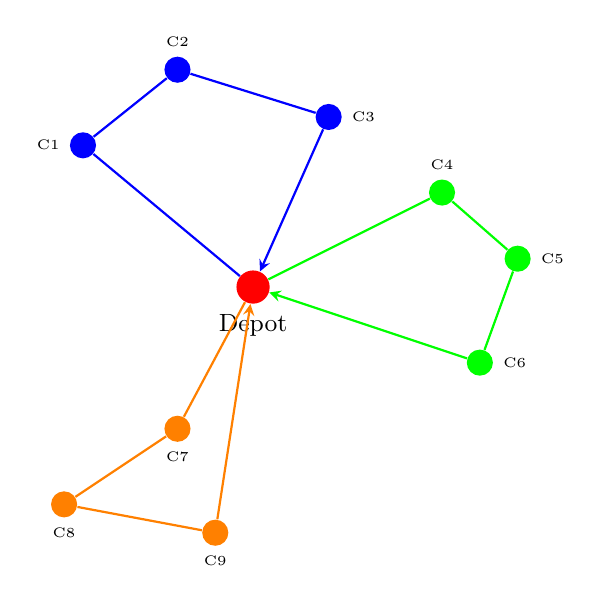
\begin{tikzpicture}[scale=1.2]

% Depot
\node[circle, fill=red, minimum size=12pt, label=below:\small Depot] (depot) at (0,0) {};

% Route 1 (Blue)
\node[circle, fill=blue, minimum size=8pt, label=left:\tiny C1] (c1) at (-1.8,1.5) {};
\node[circle, fill=blue, minimum size=8pt, label=above:\tiny C2] (c2) at (-0.8,2.3) {};
\node[circle, fill=blue, minimum size=8pt, label=right:\tiny C3] (c3) at (0.8,1.8) {};

% Route 2 (Green)
\node[circle, fill=green, minimum size=8pt, label=above:\tiny C4] (c4) at (2,1) {};
\node[circle, fill=green, minimum size=8pt, label=right:\tiny C5] (c5) at (2.8,0.3) {};
\node[circle, fill=green, minimum size=8pt, label=right:\tiny C6] (c6) at (2.4,-0.8) {};

% Route 3 (Orange)
\node[circle, fill=orange, minimum size=8pt, label=below:\tiny C7] (c7) at (-0.8,-1.5) {};
\node[circle, fill=orange, minimum size=8pt, label=below:\tiny C8] (c8) at (-2,-2.3) {};
\node[circle, fill=orange, minimum size=8pt, label=below:\tiny C9] (c9) at (-0.4,-2.6) {};

% Edges
\draw[blue, thick, ->, >=stealth] (depot) -- (c1) -- (c2) -- (c3) -- (depot);
\draw[green, thick, ->, >=stealth] (depot) -- (c4) -- (c5) -- (c6) -- (depot);
\draw[orange, thick, ->, >=stealth] (depot) -- (c7) -- (c8) -- (c9) -- (depot);

\end{tikzpicture}
\end{center}

\end{columns}
\end{frame}


\begin{frame}{Proving CVRP is NP-Hard}
\begin{block}{Our Approach}
We prove CVRP is NP-Hard by showing a polynomial-time reduction from the Traveling Salesman Problem (TSP).
\end{block}

\vspace{0.5cm}

\begin{columns}[T]
\column{0.48\textwidth}
\centering
\textbf{Known:}\\
TSP is NP-Hard

\column{0.48\textwidth}
\centering
\textbf{To Prove:}\\
CVRP is NP-Hard
\end{columns}

\vspace{0.5cm}

\begin{center}
\Large
$\text{TSP} \leq_P \text{CVRP}$
\end{center}
\end{frame}

\section{Visual Reduction: TSP $\rightarrow$ CVRP}

%----------------------------------
\begin{frame}{Step 1: Traveling Salesman Problem (TSP)}
\centering

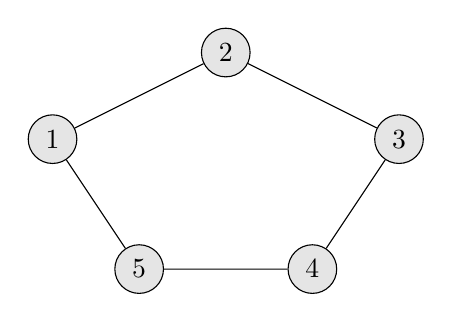
\begin{tikzpicture}[scale=1.1]

\node[circle, draw, fill=gray!20] (1) at (0,1.5) {1};
\node[circle, draw, fill=gray!20] (2) at (2,2.5) {2};
\node[circle, draw, fill=gray!20] (3) at (4,1.5) {3};
\node[circle, draw, fill=gray!20] (4) at (3,0) {4};
\node[circle, draw, fill=gray!20] (5) at (1,0) {5};

\draw (1)--(2)--(3)--(4)--(5)--(1);

\end{tikzpicture}

\vspace{1em}
\footnotesize
All nodes are identical — find a minimum Hamiltonian cycle
\end{frame}

%----------------------------------
\begin{frame}{Step 2: Choose a Depot}
\centering

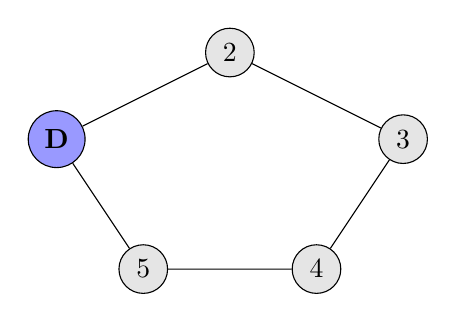
\begin{tikzpicture}[scale=1.1]

\node[circle, draw, fill=blue!40] (D) at (0,1.5) {\textbf{D}};
\node[circle, draw, fill=gray!20] (2) at (2,2.5) {2};
\node[circle, draw, fill=gray!20] (3) at (4,1.5) {3};
\node[circle, draw, fill=gray!20] (4) at (3,0) {4};
\node[circle, draw, fill=gray!20] (5) at (1,0) {5};

\draw (D)--(2)--(3)--(4)--(5)--(D);

\end{tikzpicture}

\vspace{1em}
\footnotesize
Select any node as the depot
\end{frame}

%----------------------------------
\begin{frame}{Building the CVRP Instance (from TSP)}
\centering

\begin{tikzpicture}[scale=1.05]

%---------------- Graph ----------------
\node[circle, draw, fill=blue!40] (D) at (0,1.5) {\textbf{D}};
\node[circle, draw, fill=green!40] (2) at (2,2.5) {2};
\node[circle, draw, fill=green!40] (3) at (4,1.5) {3};
\node[circle, draw, fill=green!40] (4) at (3,0) {4};
\node[circle, draw, fill=green!40] (5) at (1,0) {5};

\draw (D)--(2)--(3)--(4)--(5)--(D);

%---------------- Demand Labels ----------------
\only<2->{
\node[above] at (2.north) {$d=1$};
\node[above] at (3.north) {$d=1$};
\node[right] at (4.east) {$d=1$};
\node[left] at (5.west) {$d=1$};
}

%---------------- Route ----------------
\only<3->{
\draw (D)--(2)--(3)--(4)--(5)--(D);
}

%---------------- Variable Box ----------------
\node[varbox, right=3cm of 3] {
\textbf{CVRP Parameters}\\[0.3em]
\only<1->{Customers: n - 1\\}
\only<2->{Demand: $d_i = 1$\\}
\only<3->{Vehicles: $m = 1$\\}
\only<4->{Capacity: $Q = n-1$}
};

\end{tikzpicture}

\vspace{0.8em}
\footnotesize
\only<1>{Define customers}
\only<2>{Assign unit demands}
\only<3>{Restrict to one vehicle}
\only<4>{Capacity forces a single tour}
\end{frame}

%----------------------------------
\begin{frame}{Key Insight}
\begin{block}{Crucial Observation}
By setting
\[
vehicles = 1, \quad demand = 1, \quad capacity = n-1
\]
\end{block}

\begin{block}{Equivalence}
One CVRP route visiting all customers  
$\Longleftrightarrow$  
One TSP Hamiltonian cycle
\end{block}
\end{frame}

%----------------------------------
\begin{frame}{NP-Hardness Conclusion}
\[
\text{TSP} \;\leq_p\; \text{CVRP}
\]

\vspace{1em}

\begin{block}{Conclusion}
Since TSP is NP-Hard, the Capacitated Vehicle Routing Problem is NP-Hard.
\end{block}
\end{frame}

\section{Taxonomy of Algorithms}

\begin{frame}[allowframebreaks]{Algorithm Categories Defined}
    Before detailing specific CVRP algorithms, we must define the classes of algorithms used in operations research.
    
    \vspace{1em}
    \textbf{1. Exact Algorithms}
    \begin{itemize}
        \item \textbf{Definition:} Algorithms that guarantee finding the \textit{globally optimal} solution.
        \item \textbf{Pros:} Proof of optimality.
        \item \textbf{Cons:} Exponential time complexity ($O(2^n)$ or worse). Only feasible for small instances ($n < 200$).
    \end{itemize}

    \framebreak

    \textbf{2. Approximation Algorithms}
    \begin{itemize}
        \item \textbf{Definition:} Polynomial-time algorithms that provide a guarantee on the solution quality.
        \item \textbf{The Guarantee ($\alpha$):} An algorithm is an $\alpha$-approximation if for any instance, the solution $Sol \le \alpha \times Opt$.
        \item \textbf{Context:} For general CVRP, finding a constant factor approximation is difficult due to the hardness of Bin Packing.
    \end{itemize}

    \framebreak

    \textbf{3. Heuristics}
    \begin{itemize}
        \item \textbf{Definition:} "Rule of thumb" techniques. They use problem-specific knowledge to find "good enough" solutions quickly.
        \item \textbf{No Guarantees:} Unlike approximation algorithms, they do not guarantee a bound on the error.
        \item \textbf{Types:}
        \begin{itemize}
            \item \textit{Constructive:} Build a solution from scratch.
            \item \textit{Improvement:} Take an existing solution and try to make it better.
        \end{itemize}
    \end{itemize}

    \framebreak

    \textbf{4. Metaheuristics}
    \begin{itemize}
        \item \textbf{Definition:} High-level problem-independent frameworks that guide local search heuristics to escape local optima.
        \item \textbf{Mechanism:} They balance \textit{Exploration} (searching new areas of the solution space) and \textit{Exploitation} (refining the current best solution).
        \item \textbf{Examples:} Genetic Algorithms, Tabu Search, Simulated Annealing.
    \end{itemize}
\end{frame}

\begin{frame}{Existing Algorithms}
\resizebox{\textwidth}{!}{%
  \begin{tabular}{l l l}
    \toprule
    \textbf{Category} & \textbf{Algorithm} & \textbf{Key Features} \\
    \midrule
    \textbf{Exact} & Branch and Bound \cite{laporte1983branch} & Enumerates candidate solutions by forming a rooted tree \\ & \textbf{Branch-and-Cut} \cite{augerat1995computational} & Uses capacity cuts and comb inequalities. \\
                   & Branch-Cut-and-Price \cite{fukasawa2006robust} & State-of-the-art; uses Column Generation. \\
    \midrule
    \textbf{Approximation} & Christofides' Ext. \cite{christofides1979set} & Extensions of TSP approx; mostly theoretical. \\
    \midrule
    \textbf{Heuristic} & Clarke \& Wright \cite{shour2015modified} & Greedy merging based on "savings" ($s_{ij}$). \\
                       & \textbf{Sweep Algorithm} \cite{sehta2021sweep} & Clusters by polar angle, solves TSP per cluster. \\
    \midrule
    \textbf{Metaheuristic} & Tabu Search \cite{barbarosoglu1999tabu} & Local search with memory structures. \\
                           & \textbf{Genetic Algorithm} \cite{jasim2024guided} & Population-based; often uses "Giant Tour" split. \\
                           & Large Neighborhood Search \cite{gu2019adaptive} & Destroy part of the solution and recreate it \\
    \bottomrule
  \end{tabular}
}
\end{frame}


% -----------------------------------------------------------------------------
% SECTION 4: EXACT ALGORITHMS
% -----------------------------------------------------------------------------
\section{Exact Algorithms for CVRP}

\begin{frame}{Branch and Bound (B\&B)}
    \textbf{Concept:} 
    Systematically enumerates candidate solutions by forming a rooted tree \cite{laporte1983branch}.
    
    \textbf{Mechanism:}
    \begin{enumerate}
        \item \textbf{Branching:} Splits the problem into smaller subproblems (e.g., "Edge $x_{12}$ must be used" vs "Edge $x_{12}$ cannot be used").
        \item \textbf{Bounding:} Calculates a lower bound for each subproblem (usually via Linear Relaxation).
        \item \textbf{Pruning:} If a subproblem's Lower Bound $>$ Current Best Solution, that branch is discarded (pruned).
    \end{enumerate}
\end{frame}

\begin{frame}{Branch and Cut (B\&C)}
    \textbf{Enhancement to B\&B:}
    Standard B\&B is weak because the Linear Relaxation of CVRP is often too loose. B\&C adds \textit{Valid Inequalities} (Cuts) to tighten the relaxation \cite{augerat1995computational}.
    
    \textbf{Famous Cuts:}
    \begin{itemize}
        \item \textbf{Rounded Capacity Cuts:} Ensures demand constraints are met for subsets.
        \item \textbf{Comb Inequalities:} Generalized from TSP to handle connectivity.
        \item \textbf{Framed Capacity Cuts:} Specific to VRP, combining capacity and geometric constraints.
    \end{itemize}
    \textit{Status:} Currently effective for $n \approx 100-150$.
\end{frame}

\begin{frame}{Branch-Cut-and-Price (BCP)}
    \textbf{The State-of-the-Art:}
    Combines Branch-and-Bound with \textbf{Column Generation} \cite{fukasawa2006robust}.
    
    \textbf{Set Partitioning Formulation:}
    Instead of deciding edges ($x_{ij}$), we decide which \textit{Routes} ($r_k$) to select.
    $$ \min \sum_{r \in \Omega} c_r \lambda_r $$
    Subject to: Each customer is in exactly one route.
    
    \textbf{Column Generation:}
    Since the set of possible routes $\Omega$ is exponential, we start with a few. We generate new "promising" routes dynamically by solving a \textbf{Pricing Subproblem} (usually a Shortest Path Problem with Resource Constraints - SPPRC).
    
    \textit{Status:} Can solve instances up to $n \approx 200-300$.
\end{frame}

% -----------------------------------------------------------------------------
% SECTION 5: HEURISTIC ALGORITHMS
% -----------------------------------------------------------------------------
\section{Classical Heuristic Algorithms}

\begin{frame}{Constructive Heuristics}
    These algorithms build a feasible solution from scratch.
    
    \textbf{A. Clarke and Wright Savings Algorithm} \cite{shour2015modified}
    \begin{itemize}
        \item \textbf{Init:} $n$ routes ($0 \to i \to 0$).
        \item \textbf{Metric:} Savings $s_{ij} = c_{i0} + c_{0j} - c_{ij}$.
        \item \textbf{Step:} Merge routes with max $s_{ij}$ if capacity allows.
        \item \textbf{Complexity:} $O(n^2 \log n)$.
    \end{itemize}
    
    \textbf{B. Sweep Algorithm} \cite{sehta2021sweep}
    \begin{itemize}
        \item \textbf{Geometric approach.}
        \item Sort customers by polar angle around the depot.
        \item "Sweep" around, adding customers to a vehicle until capacity $Q$ is full, then start a new vehicle.
        \item Solve TSP for each cluster.
    \end{itemize}
\end{frame}

% \begin{frame}{Improvement Heuristics (Local Search)}
%     These start with a solution and iteratively improve it.
    
%     \textbf{Intra-Route Moves (TSP-like)}
%     \begin{itemize}
%         \item \textbf{2-Opt:} Remove two edges, reconnect to uncross lines.
%         \item \textbf{Or-Opt:} Move a chain of 3 consecutive nodes to a different position.
%     \end{itemize}
    
%     \textbf{Inter-Route Moves (VRP-specific)}
%     \begin{itemize}
%         \item \textbf{Relocate:} Move customer $i$ from Route A to Route B.
%         \item \textbf{Swap:} Exchange customer $i$ (Route A) with customer $j$ (Route B).
%         \item \textbf{Cross:} Exchange the tails of two routes.
%     \end{itemize}
% \end{frame}

% -----------------------------------------------------------------------------
% SECTION 6: METAHEURISTICS
% -----------------------------------------------------------------------------
\section{Metaheuristic Algorithms}

\begin{frame}{Tabu Search (TS)}
    \textbf{Mechanism:} \cite{barbarosoglu1999tabu}
    \begin{itemize}
        \item Performs local search (like Swap/Relocate).
        \item \textbf{The Tabu List:} To prevent cycling (A $\to$ B $\to$ A), recent moves are declared "Tabu" (forbidden) for a certain number of iterations.
        \item \textbf{Aspiration Criterion:} Can override Tabu status if the move produces a new global best solution.
    \end{itemize}
\end{frame}

\begin{frame}{Genetic Algorithms (GA)}
    \textbf{Biological Analogy:} Evolution \cite{jasim2024guided}.
    \begin{itemize}
        \item \textbf{Population:} A set of solutions (Chromosomes).
        \item \textbf{Crossover:} Combine parents to create offspring (e.g., Order Crossover).
        \item \textbf{Mutation:} Randomly tweak a child to maintain diversity.
        \item \textbf{Selection:} Survival of the fittest.
    \end{itemize}
    \textbf{VRP Specialization:}
    Most successful VRP GAs use a \textbf{"Giant Tour"} representation (a single sequence of all customers) and a \textbf{Split Algorithm} to optimally break the sequence into routes.
\end{frame}

\begin{frame}{Ant Colony Optimization (ACO)}
    \textbf{Biological Analogy:} Foraging ants \cite{stodola2014aco}.
    \begin{itemize}
        \item \textbf{Pheromones:} Artificial agents (ants) construct routes probabilistically based on "pheromone trails" $\tau_{ij}$ on edges.
        \item \textbf{Update:} Good routes receive more pheromone; unused edges evaporate.
        \item \textbf{Result:} Over time, the colony converges on the optimal path.
    \end{itemize}
\end{frame}

\begin{frame}{Large Neighborhood Search (LNS)}
    \textbf{Mechanism:} Ruin and Recreate \cite{gu2019adaptive}.
    \begin{itemize}
        \item \textbf{Ruin:} Intentionally destroy part of the solution (e.g., remove 20\% of customers randomly or spatially).
        \item \textbf{Recreate:} Re-insert the removed customers using a greedy heuristic or regret heuristic.
        \item \textbf{ALNS (Adaptive LNS):} Automatically selects which "Ruin" and "Recreate" operators work best for the current instance.
    \end{itemize}
\end{frame}

% % ---------------------------------------------------------------
\section{Implementation}
% % ---------------------------------------------------------------

\begin{frame}{Exact Algorithm Implementation}

Two independent Python implementations were developed to solve
the CVRP exactly, both tested on standard \texttt{.vrp} benchmark
instances.

\vspace{0.6em}

%----- Side-by-side comparison ------------------------------------
\begin{table}[t]
\centering
\resizebox{\textwidth}{!}{%
\begin{tabular}{lll}
\toprule
\textbf{Aspect} & \textbf{Custom B\&C} & \textbf{OR-Tools} \\
\midrule
LP / MIP engine   & \texttt{scipy} HiGHS           & OR-Tools CP engine \\
Cuts added        & Capacity + Comb                & Internal (hidden)  \\
First solution    & Nearest-neighbour + 2-opt      & Multi-strategy     \\
Improvement       & B\&B with LIFO stack           & GLS / Tabu / SA    \\
Optimality proof  & Yes (within node budget)       & Yes (time limit)   \\
Scalability       & $n \lesssim 50$                & $n \lesssim 200$   \\
Dependencies      & \texttt{numpy, scipy}          & \texttt{ortools}   \\
\bottomrule
\end{tabular}
}
\end{table}

\vspace{0.4em}
\footnotesize
Both solvers accept standard TSPLIB \texttt{.vrp} files and are
executed via the shell scripts \texttt{run\_bc.sh} and
\texttt{run\_all.sh} for batch benchmarking.

\end{frame}

% ---------------------------------------------------------------
% Results Slides (drop-in replacement for results_slide.tex)
% Requires in preamble:
  % \usepackage{booktabs}
  % \usepackage{colortbl}
  % \usepackage{xcolor}
  % \usepackage{amsmath}
  % \usepackage{graphicx}
  % \usepackage{hyperref}
%
% Place the following image files in the same folder as main.tex:
%   b&c_A-n80-k10_plot.png
%   ortools_A-n80-k10_plot.png
% ---------------------------------------------------------------

\section{Experimental Results}

% ================================================================
% FRAME 1 — Setup + Table Part 1 (instances 1–14)
% ================================================================
\begin{frame}{Results: Custom B\&C vs.\ OR-Tools \hfill {\small (1/2)}}

\begin{block}{Experimental Setup}
\small
Tested on \textbf{27 Augerat Set-A benchmarks} ($n = 31$--$79$ customers).
\textbf{Time limits:} OR-Tools $= 360\,\text{s}$,\; Custom B\&C $= 600\,\text{s}$.
Known optimal distances used as ground truth.
\end{block}

\vspace{0.3em}

\resizebox{\textwidth}{!}{%
\begin{tabular}{l r r r r r r r}
\toprule
\textbf{Instance} & \textbf{$n$} & \textbf{$k$} & \textbf{Optimal} &
\textbf{B\&C} & \textbf{B\&C Gap (\%)} &
\textbf{OR-Tools} & \textbf{ORT Gap (\%)} \\
\midrule
A-n32-k5  & 31 & 5 & 784  & 926  & 18.11 & \cellcolor{green!25}784  & \cellcolor{green!25}0.00 \\
A-n33-k5  & 32 & 5 & 661  & \cellcolor{green!25}661  & \cellcolor{green!25}0.00 & \cellcolor{green!25}661  & \cellcolor{green!25}0.00 \\
A-n33-k6  & 32 & 6 & 742  & 836  & 12.67 & \cellcolor{green!25}742  & \cellcolor{green!25}0.00 \\
A-n34-k5  & 33 & 5 & 778  & 805  &  3.47 & \cellcolor{green!25}778  & \cellcolor{green!25}0.00 \\
A-n36-k5  & 35 & 5 & 799  & 1031 & 29.04 & \cellcolor{green!25}799  & \cellcolor{green!25}0.00 \\
A-n37-k5  & 36 & 5 & 669  & 756  & 13.00 & \cellcolor{green!25}669  & \cellcolor{green!25}0.00 \\
A-n37-k6  & 36 & 6 & 949  & 1271 & 33.93 & \cellcolor{green!25}949  & \cellcolor{green!25}0.00 \\
A-n38-k5  & 37 & 5 & 730  & 986  & 35.07 & \cellcolor{green!25}730  & \cellcolor{green!25}0.00 \\
A-n39-k5  & 38 & 5 & 822  & 1028 & 25.06 & 825  & 0.36 \\
A-n39-k6  & 38 & 6 & 831  & 957  & 15.16 & 833  & 0.24 \\
A-n44-k6  & 43 & 6 & 937  & 1343 & 43.33 & 939  & 0.21 \\
A-n45-k6  & 44 & 6 & 944  & 1422 & 50.64 & 951  & 0.74 \\
A-n45-k7  & 44 & 7 & 1146 & 1383 & 20.68 & \cellcolor{green!25}1146 & \cellcolor{green!25}0.00 \\
A-n46-k7  & 45 & 7 & 914  & 1117 & 22.21 & \cellcolor{green!25}914  & \cellcolor{green!25}0.00 \\
\bottomrule
\end{tabular}
}

\vspace{0.2em}
\footnotesize
\textcolor{green!60!black}{$\blacksquare$}~Optimal reached \quad (\textit{continued on next page})

\end{frame}

% ================================================================
%         Table Part 2 (instances 15–27)
% ================================================================
\begin{frame}{Results: Custom B\&C vs.\ OR-Tools \hfill {\small (2/2)}}

\resizebox{\textwidth}{!}{%
\begin{tabular}{l r r r r r r r}
\toprule
\textbf{Instance} & \textbf{$n$} & \textbf{$k$} & \textbf{Optimal} &
\textbf{B\&C} & \textbf{B\&C Gap (\%)} &
\textbf{OR-Tools} & \textbf{ORT Gap (\%)} \\
\midrule
A-n48-k7  & 47 & 7  & 1073 & 1453 & 35.41 & \cellcolor{green!25}1073 & \cellcolor{green!25}0.00 \\
A-n53-k7  & 52 & 7  & 1010 & 1385 & 37.13 & 1017 & 0.69 \\
A-n54-k7  & 53 & 7  & 1167 & 1386 & 18.77 & 1170 & 0.26 \\
A-n55-k9  & 54 & 9  & 1073 & 1472 & 37.19 & 1074 & 0.09 \\
A-n60-k9  & 59 & 9  & 1354 & 1775 & 31.09 & \cellcolor{green!25}1354 & \cellcolor{green!25}0.00 \\
% A-n61-k9  & 60 & 9  & 1034 & 1354 & 30.95 & \cellcolor{red!20}1184 & \cellcolor{red!20}14.51 \\
A-n62-k8  & 61 & 8  & 1288 & 1713 & 33.00 & 1306 & 1.40 \\
A-n63-k10 & 62 & 10 & 1314 & 1860 & 41.55 & 1321 & 0.53 \\
A-n63-k9  & 62 & 9  & 1616 & 2139 & 32.36 & 1641 & 1.55 \\
A-n64-k9  & 63 & 9  & 1401 & 1903 & 35.83 & 1419 & 1.28 \\
A-n65-k9  & 64 & 9  & 1174 & 1694 & 44.29 & 1184 & 0.85 \\
A-n69-k9  & 68 & 9  & 1159 & 1477 & 27.44 & 1170 & 0.95 \\
A-n80-k10 & 79 & 10 & 1763 & 2290 & 29.89 & 1791 & 1.59 \\
\midrule
\textbf{Average} & & & & & \textbf{28.08} & & \textbf{1.06} \\
\bottomrule
\end{tabular}
}

\vspace{0.4em}

\begin{columns}[T]
\column{0.48\textwidth}
\begin{block}{\small Custom B\&C (limit: 600\,s)}
\footnotesize
\begin{itemize}
  \item Avg.\ gap: $\mathbf{28.08\%}$
  \item Gap range: $0\%$ -- $50.64\%$
\end{itemize}
\end{block}

\column{0.48\textwidth}
\begin{block}{\small OR-Tools (limit: 360\,s)}
\footnotesize
\begin{itemize}
  \item Avg.\ gap: $\mathbf{1.06\%}$
  \item Gap range: $0\%$ -- $1.59\%$
\end{itemize}
\end{block}
\end{columns}

\end{frame}

% ================================================================
%         Custom B&C route plot (A-n80-k10)
% ================================================================
\begin{frame}{Custom B\&C Solution — A-n80-k10}

\begin{block}{Instance: A-n80-k10 \quad $n=79$,\; $k=10$,\; Optimal $= 1763$}
B\&C result: $\mathbf{2290}$ \quad Gap: $\mathbf{29.89\%}$ \quad Time limit: $600\,\text{s}$
\end{block}

\vspace{0.2em}

\begin{center}
  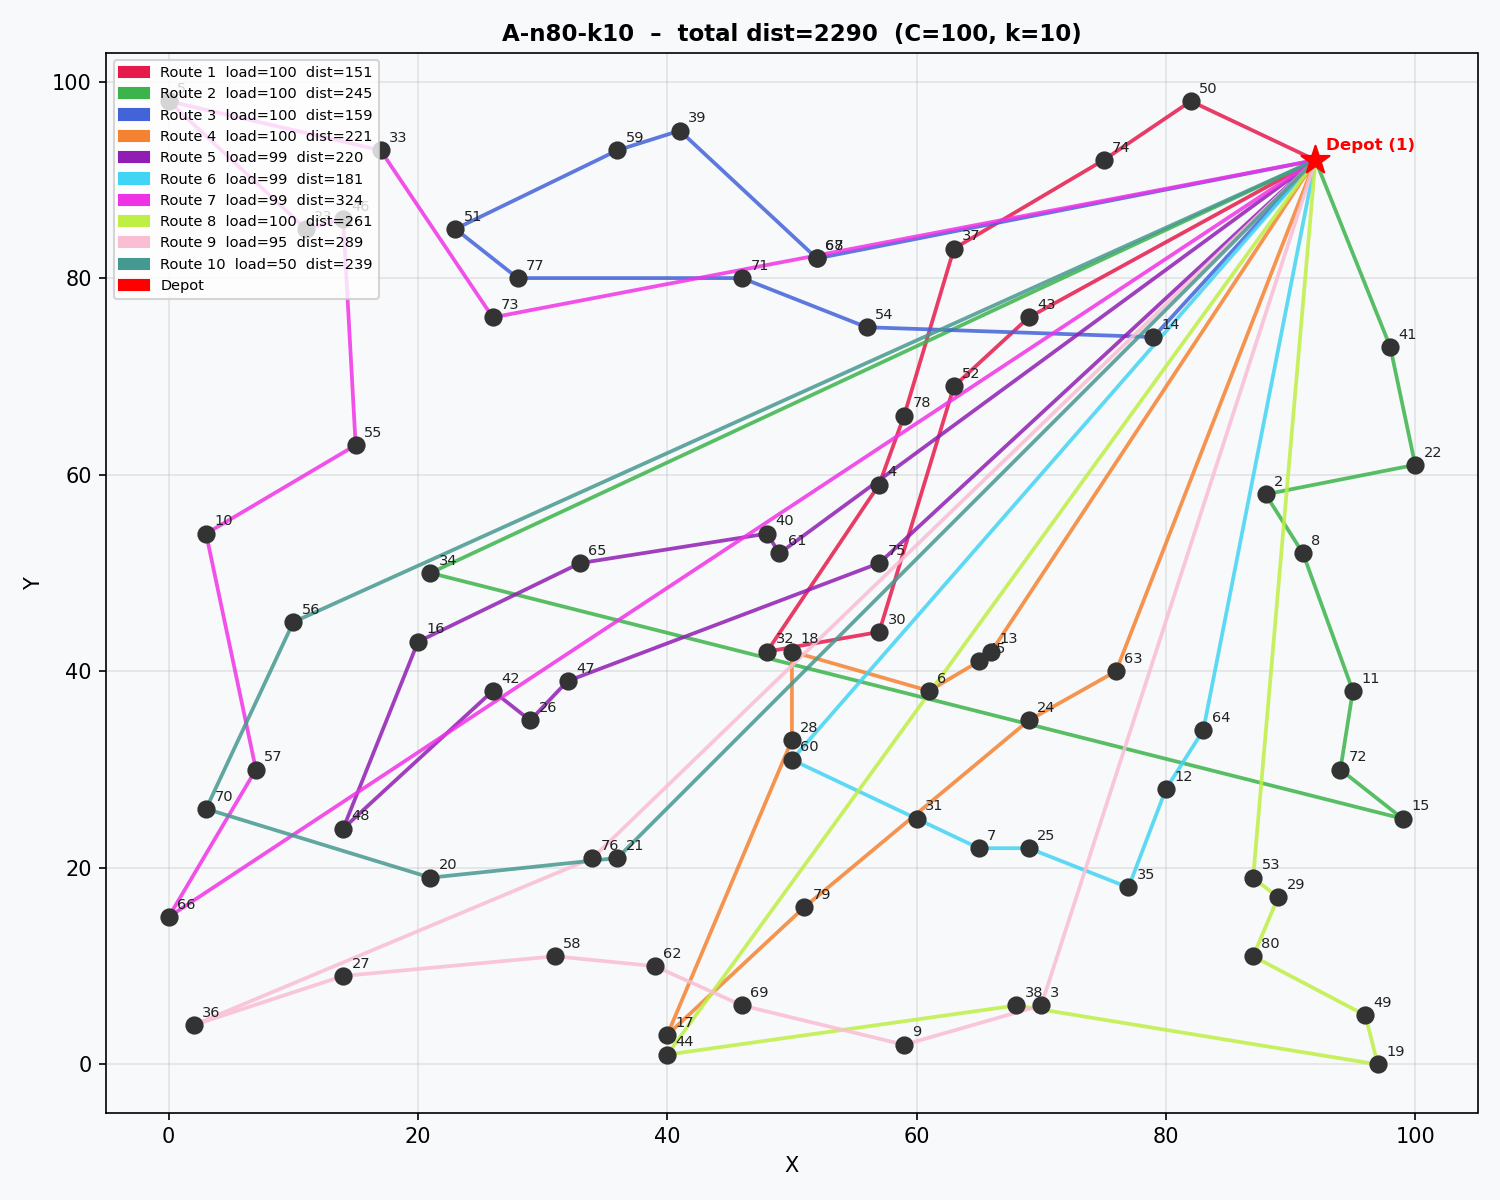
\includegraphics[width=0.75\textwidth]{b&c_A-n80-k10_plot.png}
\end{center}

\end{frame}

% ================================================================
%         OR-Tools route plot (A-n80-k10)
% ================================================================
\begin{frame}{OR-Tools Solution — A-n80-k10}

\begin{block}{Instance: A-n80-k10 \quad $n=79$,\; $k=10$,\; Optimal $= 1763$}
OR-Tools result: $\mathbf{1791}$ \quad Gap: $\mathbf{1.59\%}$ \quad Time limit: $360\,\text{s}$
\end{block}

\vspace{0.3em}

\begin{center}
  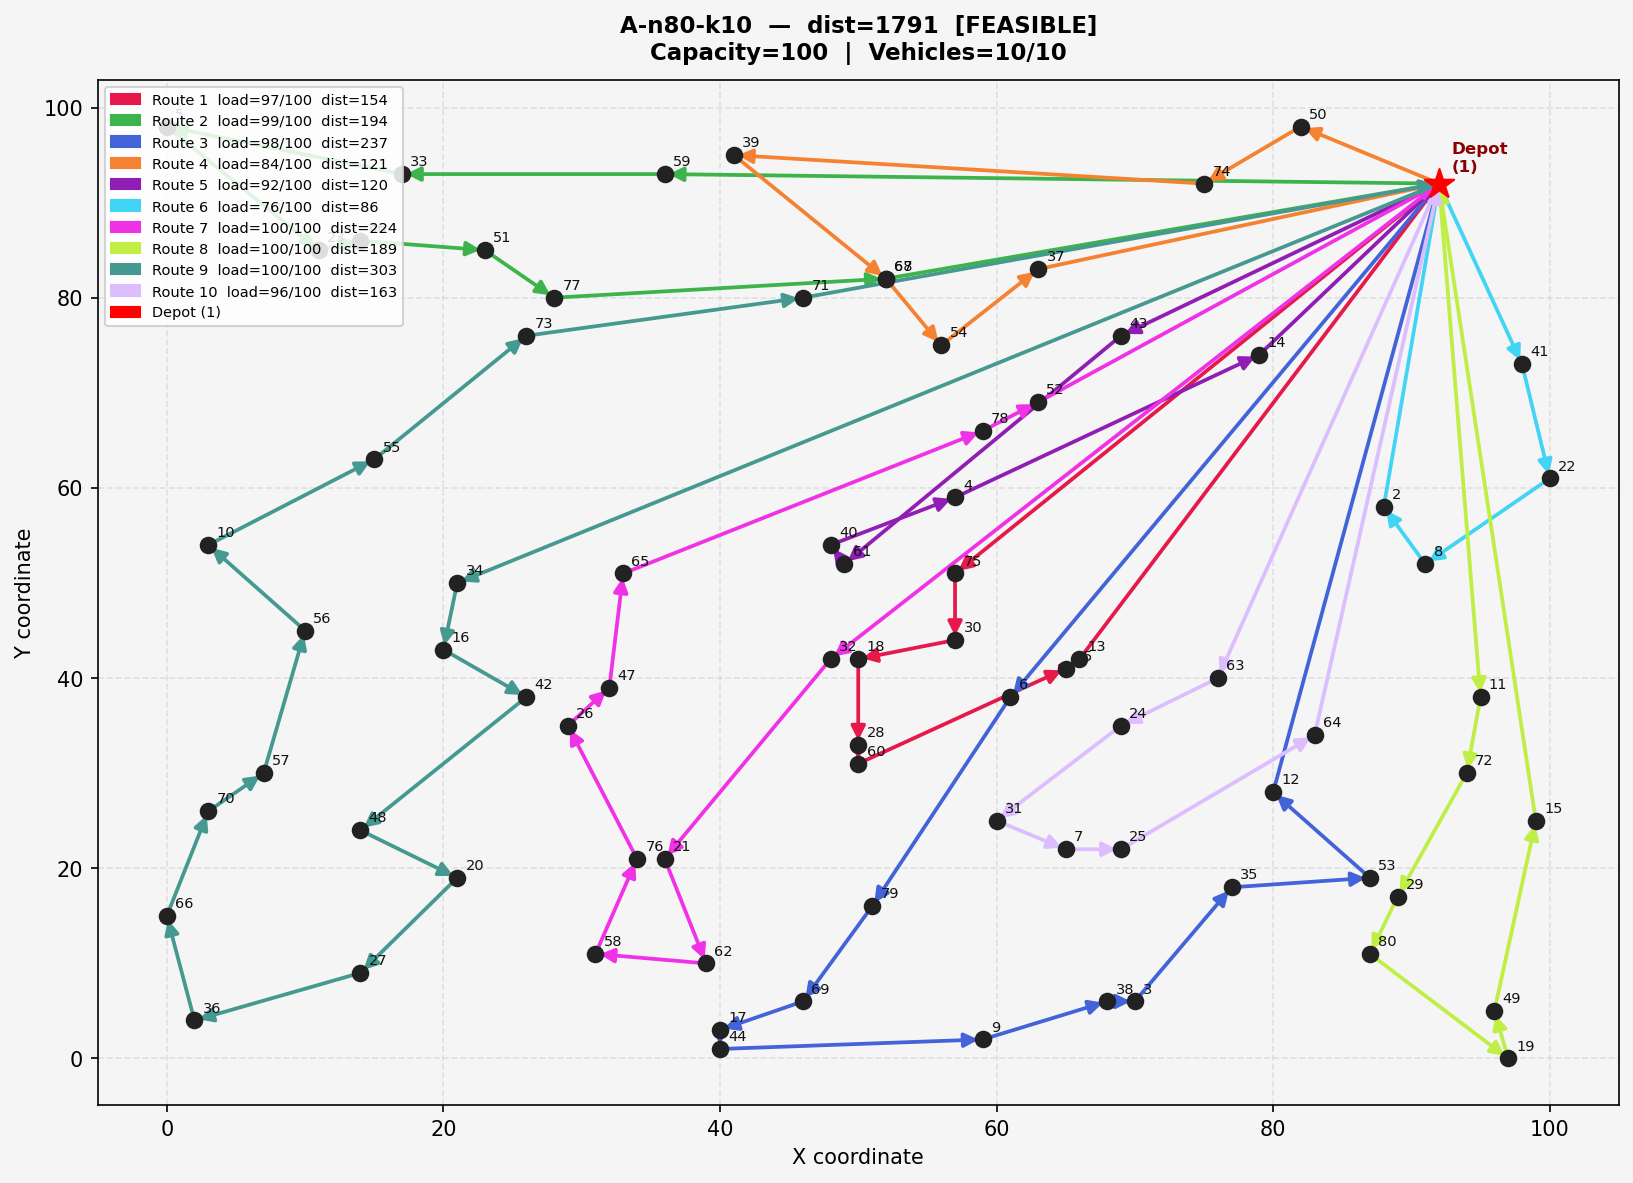
\includegraphics[width=0.75\textwidth]{ortools_A-n80-k10_plot.png}
\end{center}

\end{frame}

%==================================================================
%
%     Add slides for heuristics below:
%
%==================================================================

% ======================================================================
\section{Gillett \& Miller Sweep (\texttt{cvrp\_sweep\_gillett.py})}
% ======================================================================

% Page 4: Algorithm Overview
\begin{frame}{Gillett \& Miller Sweep — Algorithm Overview}

\begin{block}{Core Idea}
Customers are sorted by their polar angle around the depot.
A ``sweep'' groups them into vehicle routes as the angle increases,
respecting the capacity constraint $Q$.
Each cluster is then optimised as a TSP sub-tour.
\end{block}

\vspace{0.2em}

\begin{columns}[T]

\column{0.52\textwidth}
\textbf{Steps:}
\begin{enumerate}\small
  \item Compute polar angle $\theta_i = \text{atan2}(y_i - y_0,\; x_i - x_0)$ for every customer $i$
  \item Sort customers by $\theta_i \in [0, 2\pi)$
  \item Greedily assign customers to the current vehicle until $\sum d_i > Q$; then open a new vehicle
  \item For each cluster: construct a route via \textbf{nearest-neighbour} heuristic
  \item Improve each route with \textbf{2-opt}
\end{enumerate}

\column{0.44\textwidth}
\begin{center}
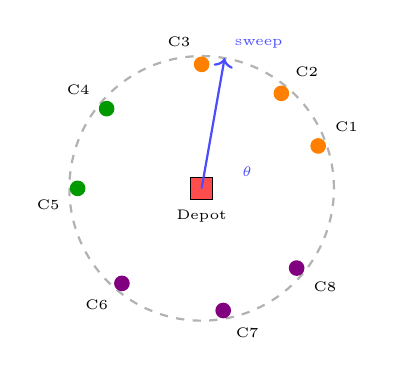
\begin{tikzpicture}[scale=1.05]
  % depot
  \node[draw, rectangle, fill=red!70, minimum size=8pt,
        label=below:\tiny Depot] (D) at (0,0) {};
  % sweep arc
  \draw[dashed, gray!60, thick] (0,0) circle (1.6cm);
  \draw[->, thick, blue!70] (0,0) -- (80:1.6) node[above right, font=\tiny]{sweep};
  % customers
  \foreach \angle/\col/\lbl in {
      20/orange/C1, 50/orange/C2, 90/orange/C3,
      140/green!60!black/C4, 180/green!60!black/C5,
      230/violet/C6, 280/violet/C7, 320/violet/C8}{
    \node[circle, fill=\col, inner sep=2pt,
          label={\angle+10}:\tiny \lbl]
      at (\angle:1.5) {};
  }
  % angle label
  \node[font=\tiny, blue!70] at (0.55,0.2) {$\theta$};
\end{tikzpicture}
\end{center}
\end{columns}

\end{frame}

% ── Worked Example slides inserted here (after Algorithm Overview) ──────

% Page 22 (moved): Problem Instance
\begin{frame}[shrink=5]{Worked Example --- Problem Instance}
\begin{columns}[T]
\column{0.44\textwidth}
\small
\textbf{Setup:}
\begin{itemize}
  \item Depot $D$ at $(5,5)$
  \item Vehicle capacity $Q = 30$
  \item 6 customers
\end{itemize}
\vspace{0.4em}
\begin{tabular}{cccc}
\toprule
Node & $(x,y)$ & $d_i$ & $\theta_i$ \\
\midrule
$D$   & $(5,5)$ & ---  & ---   \\
$C_1$ & $(2,8)$ & 10   & $135°$\\
$C_2$ & $(8,8)$ & 12   & $45°$ \\
$C_3$ & $(9,3)$ & 15   & $333°$\\
$C_4$ & $(6,1)$ & 18   & $296°$\\
$C_5$ & $(1,3)$ & 8    & $207°$\\
$C_6$ & $(3,5)$ & 14   & $180°$\\
\bottomrule
\end{tabular}
\column{0.52\textwidth}
\begin{center}
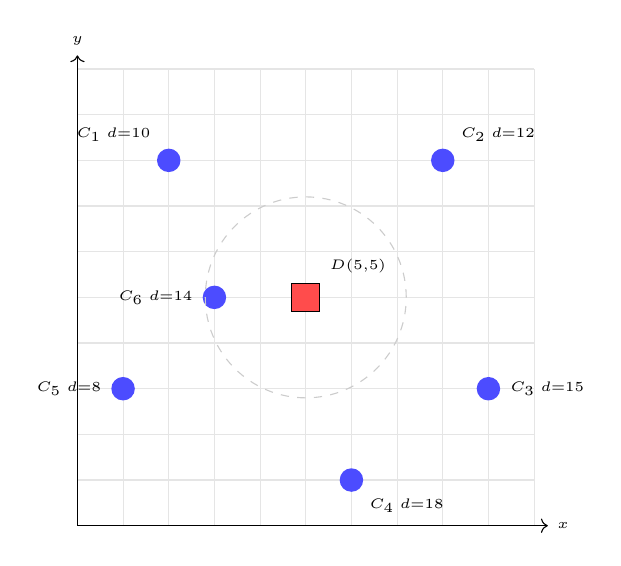
\begin{tikzpicture}[scale=0.58]
  \draw[gray!20](0,0) grid (10,10);
  \draw[->](0,0)--(10.3,0) node[right,font=\tiny]{$x$};
  \draw[->](0,0)--(0,10.3) node[above,font=\tiny]{$y$};
  \node[draw,rectangle,fill=red!70,minimum size=10pt,
        label=above right:{\tiny $D(5{,}5)$}] at (5,5){};
  \node[circle,fill=blue!70,inner sep=3pt,
        label=above left:{\tiny $C_1\;d{=}10$}] at (2,8){};
  \node[circle,fill=blue!70,inner sep=3pt,
        label=above right:{\tiny $C_2\;d{=}12$}] at (8,8){};
  \node[circle,fill=blue!70,inner sep=3pt,
        label=right:{\tiny $C_3\;d{=}15$}] at (9,3){};
  \node[circle,fill=blue!70,inner sep=3pt,
        label=below right:{\tiny $C_4\;d{=}18$}] at (6,1){};
  \node[circle,fill=blue!70,inner sep=3pt,
        label=left:{\tiny $C_5\;d{=}8$}] at (1,3){};
  \node[circle,fill=blue!70,inner sep=3pt,
        label=left:{\tiny $C_6\;d{=}14$}] at (3,5){};
  \draw[dashed,gray!40](5,5) circle(2.2);
\end{tikzpicture}
\end{center}
\end{columns}
\end{frame}

% Page 23 (moved): Sort by Polar Angle
\begin{frame}[shrink=5]{Gillett Sweep --- Step 1: Sort by Polar Angle}
\begin{block}{Polar angle from depot $D=(5,5)$}
$\theta_i = \operatorname{atan2}(y_i-5,\;x_i-5)$, mapped to $[0°,360°)$
\end{block}
\vspace{0.3em}
\begin{columns}[T]
\column{0.46\textwidth}
\small\textbf{Sorted order:}
\vspace{0.3em}
\begin{tabular}{clcc}
\toprule
Rank & Node & $\theta$ & $d_i$ \\
\midrule
1 & $C_2$ & $45°$  & 12 \\
2 & $C_1$ & $135°$ & 10 \\
3 & $C_6$ & $180°$ & 14 \\
4 & $C_5$ & $207°$ & 8  \\
5 & $C_4$ & $296°$ & 18 \\
6 & $C_3$ & $333°$ & 15 \\
\bottomrule
\end{tabular}
\column{0.50\textwidth}
\begin{center}
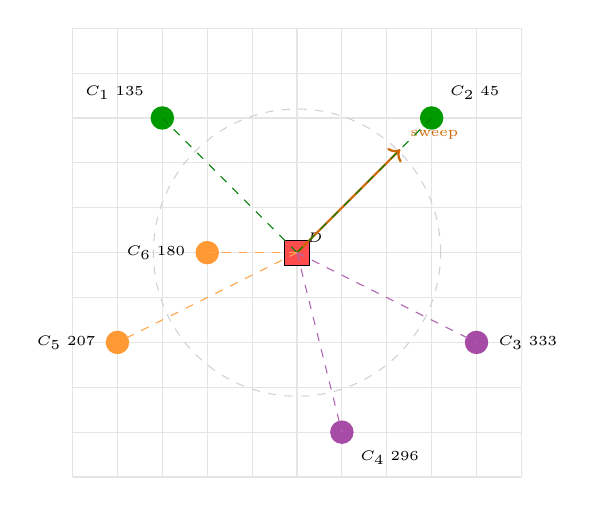
\begin{tikzpicture}[scale=0.57]
  \draw[gray!20](0,0) grid (10,10);
  \node[draw,rectangle,fill=red!70,minimum size=9pt](D) at (5,5){};
  \node[font=\tiny,above right] at (5,5){$D$};
  \draw[dashed,gray!35](5,5) circle(3.2);
  \draw[->,thick,orange!80!black](5,5)--(7.3,7.3)
       node[above right,font=\tiny]{sweep};
  \node[circle,fill=green!60!black,inner sep=3pt,
        label=above right:{\tiny $C_2\;45°$}] at (8,8){};
  \node[circle,fill=green!60!black,inner sep=3pt,
        label=above left:{\tiny $C_1\;135°$}] at (2,8){};
  \node[circle,fill=orange!80,inner sep=3pt,
        label=left:{\tiny $C_6\;180°$}] at (3,5){};
  \node[circle,fill=orange!80,inner sep=3pt,
        label=left:{\tiny $C_5\;207°$}] at (1,3){};
  \node[circle,fill=violet!70,inner sep=3pt,
        label=below right:{\tiny $C_4\;296°$}] at (6,1){};
  \node[circle,fill=violet!70,inner sep=3pt,
        label=right:{\tiny $C_3\;333°$}] at (9,3){};
  \draw[green!50!black,dashed,thin](5,5)--(8,8);
  \draw[green!50!black,dashed,thin](5,5)--(2,8);
  \draw[orange!70,dashed,thin](5,5)--(3,5);
  \draw[orange!70,dashed,thin](5,5)--(1,3);
  \draw[violet!60,dashed,thin](5,5)--(6,1);
  \draw[violet!60,dashed,thin](5,5)--(9,3);
\end{tikzpicture}
\end{center}
\end{columns}
\end{frame}

% Page 24 (moved): Greedy Clustering
\begin{frame}{Gillett Sweep --- Step 2: Greedy Clustering ($Q=30$)}
\small
Process angle-sorted customers; close a route when adding the next customer would exceed $Q$:
\vspace{0.4em}
\begin{tabular}{clccll}
\toprule
Step & Node & $d_i$ & Cum.\ load & Action & Route \\
\midrule
1 & $C_2$ & 12 & 12 & Add to V1 & \textcolor{green!60!black}{V1: $\{C_2\}$} \\
2 & $C_1$ & 10 & 22 & Add to V1 & \textcolor{green!60!black}{V1: $\{C_2,C_1\}$} \\
3 & $C_6$ & 14 & \textbf{36}$>$30 & Close V1, open V2 & \textcolor{orange!80!black}{V2: $\{C_6\}$} \\
4 & $C_5$ & 8  & 22 & Add to V2 & \textcolor{orange!80!black}{V2: $\{C_6,C_5\}$} \\
5 & $C_4$ & 18 & \textbf{40}$>$30 & Close V2, open V3 & \textcolor{violet}{V3: $\{C_4\}$} \\
6 & $C_3$ & 15 & \textbf{33}$>$30 & Close V3, open V4 & \textcolor{red!70!black}{V4: $\{C_3\}$} \\
\bottomrule
\end{tabular}
\vspace{0.4em}
\begin{block}{4 clusters formed}
\begin{columns}[T]
\column{0.24\textwidth}\centering\footnotesize
\textcolor{green!60!black}{\textbf{R1}}\\ $C_2,C_1$\\ load $=22$
\column{0.24\textwidth}\centering\footnotesize
\textcolor{orange!80!black}{\textbf{R2}}\\ $C_6,C_5$\\ load $=22$
\column{0.24\textwidth}\centering\footnotesize
\textcolor{violet}{\textbf{R3}}\\ $C_4$\\ load $=18$
\column{0.24\textwidth}\centering\footnotesize
\textcolor{red!70!black}{\textbf{R4}}\\ $C_3$\\ load $=15$
\end{columns}
\end{block}
\end{frame}

% Page 25 (moved): Nearest-Neighbour Routes
\begin{frame}{Gillett Sweep --- Step 3: Nearest-Neighbour Routes}
\begin{columns}[T]
\column{0.46\textwidth}
\small
\textbf{R1} cluster $\{C_2,C_1\}$:
\begin{enumerate}\scriptsize
  \item Start at $D(5,5)$
  \item Nearest unvisited: $C_2(8,8)$, $d{=}4.24$
  \item Nearest remaining: $C_1(2,8)$, $d{=}6.00$
  \item Return $D$: $d{=}4.24$
\end{enumerate}
\footnotesize Route: $D\!\to\!C_2\!\to\!C_1\!\to\!D$, cost $=\mathbf{14.48}$

\smallskip
\textbf{R2} cluster $\{C_6,C_5\}$:
\begin{enumerate}\scriptsize
  \item Start at $D(5,5)$
  \item Nearest: $C_6(3,5)$, $d{=}2.00$
  \item Nearest remaining: $C_5(1,3)$, $d{=}2.83$
  \item Return $D$: $d{=}4.47$
\end{enumerate}
\footnotesize Route: $D\!\to\!C_6\!\to\!C_5\!\to\!D$, cost $=\mathbf{9.30}$

\scriptsize R3: $D\!\to\!C_4\!\to\!D$, cost $=8.25$\quad
R4: $D\!\to\!C_3\!\to\!D$, cost $=8.00$

\column{0.50\textwidth}
\begin{center}
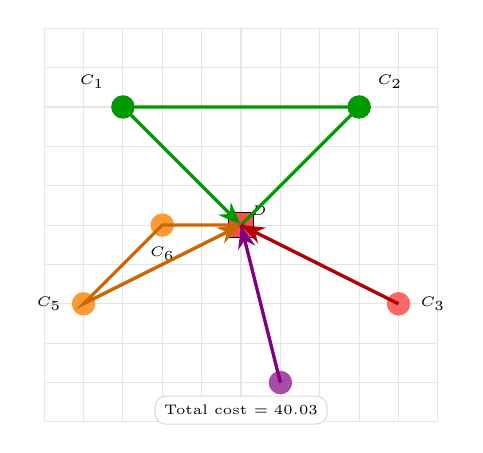
\begin{tikzpicture}[scale=0.50,>=Stealth]
  \draw[gray!20](0,0) grid (10,10);
  \node[draw,rectangle,fill=red!70,minimum size=9pt] at (5,5){};
  \node[font=\tiny,above right] at (5,5){$D$};
  \node[circle,fill=green!60!black,inner sep=3pt,
        label=above right:{\tiny $C_2$}] at (8,8){};
  \node[circle,fill=green!60!black,inner sep=3pt,
        label=above left:{\tiny $C_1$}] at (2,8){};
  \draw[->,green!60!black,very thick](5,5)--(8,8)--(2,8)--(5,5);
  \node[circle,fill=orange!80,inner sep=3pt,
        label=below:{\tiny $C_6$}] at (3,5){};
  \node[circle,fill=orange!80,inner sep=3pt,
        label=left:{\tiny $C_5$}] at (1,3){};
  \draw[->,orange!80!black,very thick](5,5)--(3,5)--(1,3)--(5,5);
  \node[circle,fill=violet!70,inner sep=3pt,
        label=below right:{\tiny $C_4$}] at (6,1){};
  \draw[->,violet,very thick](5,5)--(6,1)--(5,5);
  \node[circle,fill=red!60,inner sep=3pt,
        label=right:{\tiny $C_3$}] at (9,3){};
  \draw[->,red!70!black,very thick](5,5)--(9,3)--(5,5);
  \node[font=\tiny,fill=white,draw=gray!30,rounded corners] at (5,0.3)
       {Total cost $=40.03$};
\end{tikzpicture}
\end{center}
\end{columns}
\end{frame}

% Page 26 (moved): 2-opt Check on Route 1
\begin{frame}[shrink=8]{Gillett Sweep --- Step 4: 2-opt Check on Route 1}
\begin{columns}[T]
\column{0.50\textwidth}
\small
Route 1 after NN: $D\!\to\!C_2\!\to\!C_1\!\to\!D$

\vspace{0.4em}
Only one interior edge pair to check:
\vspace{0.2em}
\begin{tabular}{lll}
\toprule
Edges removed & Edges added & $\Delta$ \\
\midrule
$(D,C_2),(C_1,D)$ & $(D,C_1),(C_2,D)$ & \\
$4.24+4.24=8.48$ & $4.24+4.24=8.48$ & $0$ \\
\bottomrule
\end{tabular}

\vspace{0.3em}
$\Delta = 0 < \epsilon$ $\Rightarrow$ \textbf{No improvement.}

Route 1 is already 2-opt optimal (symmetric distances: order of $C_1,C_2$ does not matter when both are equidistant from depot).

\vspace{0.3em}
\begin{block}{Final Gillett solution}
\footnotesize
R1: $D\!\to\!C_2\!\to\!C_1\!\to\!D$, cost $=14.48$\\
R2: $D\!\to\!C_6\!\to\!C_5\!\to\!D$, cost $=9.30$\\
R3: $D\!\to\!C_4\!\to\!D$, cost $=8.25$\\
R4: $D\!\to\!C_3\!\to\!D$, cost $=8.00$\\
\textbf{Total $= 40.03$}
\end{block}

\column{0.46\textwidth}
\begin{center}
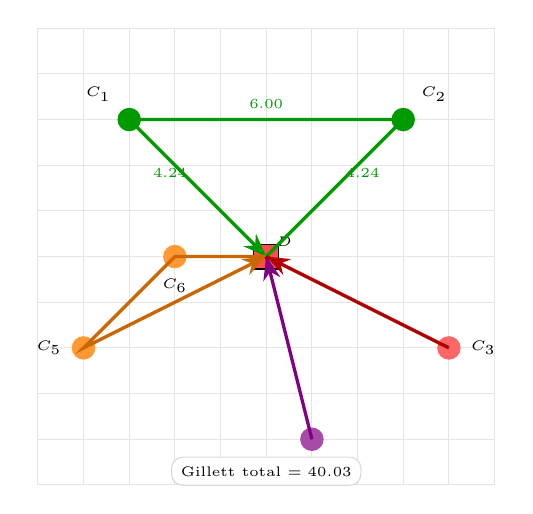
\begin{tikzpicture}[scale=0.58,>=Stealth]
  \draw[gray!20](0,0) grid (10,10);
  \node[draw,rectangle,fill=red!70,minimum size=9pt] at (5,5){};
  \node[font=\tiny,above right] at (5,5){$D$};
  % R1
  \node[circle,fill=green!60!black,inner sep=3pt,
        label=above right:{\tiny $C_2$}] at (8,8){};
  \node[circle,fill=green!60!black,inner sep=3pt,
        label=above left:{\tiny $C_1$}]  at (2,8){};
  \draw[->,green!60!black,very thick](5,5)
       --node[above right,font=\tiny]{4.24}(8,8)
       --node[above,font=\tiny]{6.00}(2,8)
       --node[above left,font=\tiny]{4.24}(5,5);
  % R2
  \node[circle,fill=orange!80,inner sep=3pt,
        label=below:{\tiny $C_6$}] at (3,5){};
  \node[circle,fill=orange!80,inner sep=3pt,
        label=left:{\tiny $C_5$}]  at (1,3){};
  \draw[->,orange!80!black,very thick](5,5)--(3,5)--(1,3)--(5,5);
  % R3,R4
  \node[circle,fill=violet!70,inner sep=3pt,
        label=below right:{\tiny $C_4$}] at (6,1){};
  \draw[->,violet,very thick](5,5)--(6,1)--(5,5);
  \node[circle,fill=red!60,inner sep=3pt,
        label=right:{\tiny $C_3$}] at (9,3){};
  \draw[->,red!70!black,very thick](5,5)--(9,3)--(5,5);
  \node[font=\tiny,fill=white,draw=gray!30,rounded corners] at (5,0.3)
       {Gillett total $=40.03$};
\end{tikzpicture}
\end{center}
\end{columns}
\end{frame}

% ======================================================================
\section{Overview of the Three Scripts}
% ======================================================================

% Page 3: Three Python Scripts — At a Glance  (extract.py column REMOVED)
\begin{frame}{Two Python Scripts — At a Glance}

\begin{columns}[T]

\column{0.48\textwidth}
\begin{block}{\small \texttt{cvrp\_sweep\_gillett.py}}
\footnotesize
\textbf{Gillett \& Miller Sweep}
\begin{itemize}
  \item Classic sweep heuristic
  \item Single-pass polar-angle clustering
  \item NN construction + 2-opt
  \item Outputs \texttt{.txt} + \texttt{.png}
\end{itemize}
\end{block}

\column{0.48\textwidth}
\begin{block}{\small \texttt{cvrp\_enhanced.py}}
\footnotesize
\textbf{Enhanced Sweep}
\begin{itemize}
  \item Multi-start sweep ($K=8$)
  \item 2-opt + Or-opt (1/2/3)
  \item Inter-route relocate \& swap
  \item Outputs \texttt{.txt} + \texttt{.png}
\end{itemize}
\end{block}

\end{columns}

\end{frame}

% ── Data structures ─────────────────────────────────────────────────────
\begin{frame}[fragile,shrink=12]{Data Structures — \texttt{Node} Class}

\begin{columns}[T]

\column{0.5\textwidth}
\begin{block}{Node}
\begin{lstlisting}
class Node:
    __slots__ = (
        "id", "x", "y",
        "demand", "angle")

    def __init__(self, id_=0,
                 x=0.0, y=0.0,
                 demand=0):
        self.id     = id_
        self.x      = x
        self.y      = y
        self.demand = demand
        self.angle  = 0.0
\end{lstlisting}
\end{block}

\column{0.46\textwidth}
\small
\textbf{Field description:}

\vspace{0.3em}
\begin{tabular}{ll}
\toprule
Field & Purpose \\
\midrule
\texttt{id}     & Node index ($1 =$ depot) \\
\texttt{x, y}   & Euclidean coordinates \\
\texttt{demand} & Delivery demand $d_i$ \\
\texttt{angle}  & Polar angle $\theta_i$ \\
\bottomrule
\end{tabular}

\vspace{0.5em}
\footnotesize
\texttt{\_\_slots\_\_} avoids a per-object dictionary, reducing memory usage for large instances.
\end{columns}

\end{frame}

% ── Geometry ────────────────────────────────────────────────────────────
\begin{frame}[fragile]{Geometry Helpers}

\begin{columns}[T]

\column{0.5\textwidth}
\begin{block}{Euclidean Distance \& Polar Angle}
\begin{lstlisting}
def euclidean(a: Node,
              b: Node) -> float:
    return math.hypot(
        a.x - b.x,
        a.y - b.y)

def polar_angle(depot: Node,
                p: Node) -> float:
    a = math.atan2(
        p.y - depot.y,
        p.x - depot.x)
    return (a + 2*math.pi
            if a < 0 else a)
\end{lstlisting}
\end{block}

\column{0.46\textwidth}
\small
\textbf{Mathematical definitions:}

\vspace{0.3em}
Euclidean distance:
\[
  d(a,b) = \sqrt{(x_a-x_b)^2 + (y_a-y_b)^2}
\]

Polar angle (mapped to $[0, 2\pi)$):
\[
  \theta_i = \operatorname{atan2}(y_i - y_0,\; x_i - x_0)
\]

\vspace{0.3em}
\footnotesize
\texttt{math.hypot} is numerically stable and avoids intermediate overflow for large coordinates.
\end{columns}

\end{frame}

% ── Nearest neighbour ───────────────────────────────────────────────────
\begin{frame}[fragile]{Nearest-Neighbour Route Construction}

\begin{columns}[T]

\column{0.54\textwidth}
\begin{block}{\texttt{nearest\_neighbour(cluster, nodes)}}
\begin{lstlisting}
def nearest_neighbour(
        cluster: list,
        nodes: list) -> list:
    remaining = list(cluster)
    route = [1]        # start at depot
    cur = 1
    while remaining:
        best_d = 1e18
        best_v = best_i = -1
        for i, v in enumerate(
                remaining):
            d = euclidean(
                nodes[cur], nodes[v])
            if d < best_d:
                best_d = d
                best_v = v
                best_i = i
        route.append(best_v)
        cur = best_v
        remaining.pop(best_i)
    route.append(1)    # return depot
    return route
\end{lstlisting}
\end{block}

\column{0.42\textwidth}
\small
\textbf{Algorithm:}
\begin{enumerate}
  \item Start at depot (node 1)
  \item Greedily visit the nearest unvisited customer
  \item Repeat until all customers in the cluster are visited
  \item Return to the depot
\end{enumerate}

\vspace{0.4em}
\textbf{Complexity:} $O(|C|^2)$ per cluster $C$

\vspace{0.4em}
\textbf{Output format:}\\
\texttt{[1, $c_1$, $c_2$, \ldots, $c_k$, 1]}\\
\footnotesize (depot at both ends)
\end{columns}

\end{frame}

% ── 2-opt ───────────────────────────────────────────────────────────────
\begin{frame}[fragile]{2-opt Improvement}

\begin{columns}[T]

\column{0.54\textwidth}
\begin{block}{\texttt{two\_opt(route, nodes)}}
\begin{lstlisting}
def two_opt(route, nodes):
    n = len(route)
    improved = True
    while improved:
        improved = False
        for i in range(1, n-2):
          for j in range(i+1, n-1):
            before = (
              euclidean(nodes[route[i-1]],
                        nodes[route[i]])
            + euclidean(nodes[route[j]],
                        nodes[route[j+1]]))
            after = (
              euclidean(nodes[route[i-1]],
                        nodes[route[j]])
            + euclidean(nodes[route[i]],
                        nodes[route[j+1]]))
            if after < before - 1e-9:
              route[i:j+1] = \
                route[i:j+1][::-1]
              improved = True
    return route
\end{lstlisting}
\end{block}

\column{0.42\textwidth}
\small
\textbf{Idea:} Remove two edges $(i{-}1,i)$ and $(j, j{+}1)$; reconnect as $(i{-}1,j)$ and $(i, j{+}1)$.

\vspace{0.3em}
\textbf{Improvement condition:}
\[
  \underbrace{d_{i-1,i} + d_{j,j+1}}_{\text{before}}
  > \underbrace{d_{i-1,j} + d_{i,j+1}}_{\text{after}}
\]

\vspace{0.3em}
\textbf{Complexity:} $O(n^2)$ per pass; repeats until no improvement.

\vspace{0.3em}
\begin{center}
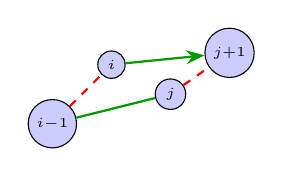
\begin{tikzpicture}[scale=0.75, >=Stealth]
  \node[circle,draw,fill=blue!20,inner sep=2pt] (a) at (0,1)   {\tiny $i{-}1$};
  \node[circle,draw,fill=blue!20,inner sep=2pt] (b) at (1,2)   {\tiny $i$};
  \node[circle,draw,fill=blue!20,inner sep=2pt] (c) at (2,1.5) {\tiny $j$};
  \node[circle,draw,fill=blue!20,inner sep=2pt] (d) at (3,2.2) {\tiny $j{+}1$};
  \draw[red,dashed,thick] (a)--(b) (c)--(d);
  \draw[green!60!black,thick,->] (a)--(c) (b)--(d);
\end{tikzpicture}
\end{center}
\footnotesize Red $=$ removed, Green $=$ added.
\end{columns}

\end{frame}

% ── Sweep clustering & solve ────────────────────────────────────────────
\begin{frame}[fragile,shrink=10]{Sweep Clustering \& Route Building}

\begin{columns}[T]

\column{0.54\textwidth}
\begin{block}{\texttt{solve(nodes, dimension, capacity)}}
\begin{lstlisting}
# Compute polar angles
customers = []
for i in range(2, dimension+1):
    nodes[i].angle = polar_angle(
        depot, nodes[i])
    customers.append(nodes[i])

# Sort by angle
customers.sort(
    key=lambda c: c.angle)

# Greedy capacity clustering
clusters, cur, load = [], [], 0
for c in customers:
    if load + c.demand <= capacity:
        cur.append(c.id)
        load += c.demand
    else:
        if cur: clusters.append(cur)
        cur, load = [c.id], c.demand
if cur: clusters.append(cur)

# Build and improve routes
routes = []
for cl in clusters:
    r = nearest_neighbour(cl, nodes)
    r = two_opt(r, nodes)
    routes.append(r)
\end{lstlisting}
\end{block}

\column{0.42\textwidth}
\small
\textbf{Clustering rule:}

Add customer $c$ to current route if:
\[
  \text{load} + d_c \leq Q
\]
Otherwise, close the current route and open a new one.

\vspace{0.5em}
\textbf{Pipeline per cluster:}
\[
  \text{cluster} \xrightarrow{\text{NN}} \text{route}
                 \xrightarrow{\text{2-opt}} \text{improved route}
\]

\vspace{0.4em}
\textbf{Total complexity:}\\
$O(n \log n)$ for sorting\\
$O(n^2)$ dominated by 2-opt\\
\end{columns}

\end{frame}

% ======================================================================
\section{Enhanced Sweep (\texttt{cvrp\_enhanced.py})}
% ======================================================================

% Page 11: Enhanced Sweep — Motivation & Design
\begin{frame}{Enhanced Sweep — Motivation \& Design}

\begin{block}{Why ``Enhanced''?}
The classic Gillett--Miller sweep is fast but sensitive to the starting
angle. A single sweep may miss good clusterings. The enhanced solver
addresses this with multi-start and richer local search.
\end{block}

\vspace{0.3em}

\begin{columns}[T]

\column{0.48\textwidth}
\textbf{Gillett--Miller (baseline):}
\begin{enumerate}\small
  \item 1 starting angle (0)
  \item NN + 2-opt per cluster
  \item No inter-route improvement
\end{enumerate}

\column{0.48\textwidth}
\textbf{Enhanced sweep (this work):}
\begin{enumerate}\small
  \item $K=8$ starting angles ($0, \frac{2\pi}{8}, \ldots$)
  \item NN + 2-opt + Or-opt (1/2/3) per cluster
  \item Inter-route \textbf{relocate} (up to 20 passes)
  \item Inter-route \textbf{swap} (up to 20 passes)
\end{enumerate}
\end{columns}

\vspace{0.3em}
\begin{center}
\small\textbf{Enhancement pipeline:}\\[0.2em]
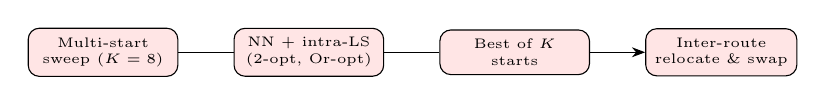
\begin{tikzpicture}[>=Stealth, node distance=0.7cm,
    box/.style={draw, rounded corners, fill=red!10,
                minimum width=1.9cm, minimum height=0.5cm,
                font=\tiny, align=center}]
  \node[box] (ms)  {Multi-start\\sweep ($K=8$)};
  \node[box] (nn)  [right=of ms]  {NN + intra-LS\\(2-opt, Or-opt)};
  \node[box] (best)[right=of nn]  {Best of $K$\\starts};
  \node[box] (ir)  [right=of best]{Inter-route\\relocate \& swap};
  \draw[->] (ms)--(nn) (nn)--(best) (best)--(ir);
\end{tikzpicture}
\end{center}

\end{frame}

% ── Enhanced Sweep worked example slides inserted here ──────────────────

% Page 27 (moved): Enhanced Sweep — Multi-Start: Different Clusterings
\begin{frame}{Enhanced Sweep --- Multi-Start: Different Clusterings}
\small Different sweep origins re-order customers, changing which clusters form.
\vspace{0.3em}
\begin{columns}[T]
\column{0.52\textwidth}
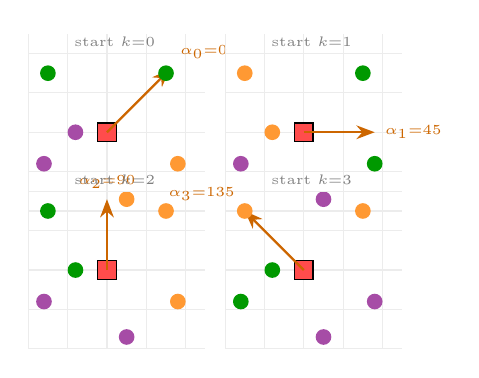
\begin{tikzpicture}[scale=0.50,>=Stealth]
  % k=0 (top-left)
  \begin{scope}[xshift=0cm,yshift=3.5cm]
    \draw[gray!15](0,0) grid (4.5,4.5);
    \node[draw,rectangle,fill=red!70,minimum size=6pt] at (2,2){};
    \draw[->,orange!80!black,thick](2,2)--(3.6,3.6)
         node[above right,font=\tiny]{$\alpha_0{=}0°$};
    \node[circle,fill=green!60!black,inner sep=2pt] at (3.5,3.5){};
    \node[circle,fill=green!60!black,inner sep=2pt] at (0.5,3.5){};
    \node[circle,fill=orange!80,inner sep=2pt]      at (3.8,1.2){};
    \node[circle,fill=orange!80,inner sep=2pt]      at (2.5,0.3){};
    \node[circle,fill=violet!70,inner sep=2pt]      at (0.4,1.2){};
    \node[circle,fill=violet!70,inner sep=2pt]      at (1.2,2.0){};
    \node[font=\tiny,gray] at (2.2,4.3){start $k{=}0$};
  \end{scope}
  % k=1 (top-right)
  \begin{scope}[xshift=5cm,yshift=3.5cm]
    \draw[gray!15](0,0) grid (4.5,4.5);
    \node[draw,rectangle,fill=red!70,minimum size=6pt] at (2,2){};
    \draw[->,orange!80!black,thick](2,2)--(3.8,2.0)
         node[right,font=\tiny]{$\alpha_1{=}45°$};
    \node[circle,fill=green!60!black,inner sep=2pt] at (3.5,3.5){};
    \node[circle,fill=green!60!black,inner sep=2pt] at (3.8,1.2){};
    \node[circle,fill=orange!80,inner sep=2pt]      at (0.5,3.5){};
    \node[circle,fill=orange!80,inner sep=2pt]      at (1.2,2.0){};
    \node[circle,fill=violet!70,inner sep=2pt]      at (2.5,0.3){};
    \node[circle,fill=violet!70,inner sep=2pt]      at (0.4,1.2){};
    \node[font=\tiny,gray] at (2.2,4.3){start $k{=}1$};
  \end{scope}
  % k=2 (bottom-left)
  \begin{scope}[xshift=0cm,yshift=0cm]
    \draw[gray!15](0,0) grid (4.5,4.5);
    \node[draw,rectangle,fill=red!70,minimum size=6pt] at (2,2){};
    \draw[->,orange!80!black,thick](2,2)--(2.0,3.8)
         node[above,font=\tiny]{$\alpha_2{=}90°$};
    \node[circle,fill=green!60!black,inner sep=2pt] at (0.5,3.5){};
    \node[circle,fill=green!60!black,inner sep=2pt] at (1.2,2.0){};
    \node[circle,fill=orange!80,inner sep=2pt]      at (3.5,3.5){};
    \node[circle,fill=orange!80,inner sep=2pt]      at (3.8,1.2){};
    \node[circle,fill=violet!70,inner sep=2pt]      at (0.4,1.2){};
    \node[circle,fill=violet!70,inner sep=2pt]      at (2.5,0.3){};
    \node[font=\tiny,gray] at (2.2,4.3){start $k{=}2$};
  \end{scope}
  % k=3 (bottom-right)
  \begin{scope}[xshift=5cm,yshift=0cm]
    \draw[gray!15](0,0) grid (4.5,4.5);
    \node[draw,rectangle,fill=red!70,minimum size=6pt] at (2,2){};
    \draw[->,orange!80!black,thick](2,2)--(0.5,3.5)
         node[above left,font=\tiny]{$\alpha_3{=}135°$};
    \node[circle,fill=green!60!black,inner sep=2pt] at (1.2,2.0){};
    \node[circle,fill=green!60!black,inner sep=2pt] at (0.4,1.2){};
    \node[circle,fill=orange!80,inner sep=2pt]      at (0.5,3.5){};
    \node[circle,fill=orange!80,inner sep=2pt]      at (3.5,3.5){};
    \node[circle,fill=violet!70,inner sep=2pt]      at (3.8,1.2){};
    \node[circle,fill=violet!70,inner sep=2pt]      at (2.5,0.3){};
    \node[font=\tiny,gray] at (2.2,4.3){start $k{=}3$};
  \end{scope}
\end{tikzpicture}
\column{0.44\textwidth}
\footnotesize
Each panel shows 4 of the 8 starts. Colours represent different vehicle assignments.

\vspace{0.4em}
After all $K=8$ starts, the solver keeps the clustering with the \textbf{lowest intra-route cost} and proceeds to inter-route improvement.

\vspace{0.4em}
\begin{block}{Why multi-start matters}
A bad sweep angle can put distant customers in the same vehicle. Trying 8 angles greatly reduces this risk on real instances.
\end{block}
\end{columns}
\end{frame}

% Page 28 (moved): Enhanced Sweep — Or-opt(1) on Route 2
\begin{frame}{Enhanced Sweep --- Or-opt(1) on Route 2}
\begin{columns}[T]
\column{0.52\textwidth}
\small
Route 2 after NN: $D\!\to\!C_6\!\to\!C_5\!\to\!D$

\vspace{0.2em}
\textbf{Or-opt(1):} try relocating $C_6$ to after $C_5$:

\footnotesize
\begin{align*}
  g_{\text{rem}} &= d(D,C_6)+d(C_6,C_5)-d(D,C_5)\\
                 &= 2.00+2.83-4.47 = 0.36\\[4pt]
  g_{\text{ins}} &= d(C_5,C_6)+d(C_6,D)-d(C_5,D)\\
                 &= 2.83+2.00-4.47 = 0.36
\end{align*}
\small
Net gain $= 0.36 - 0.36 = 0 < \epsilon$ $\Rightarrow$ \textbf{No move.}

\vspace{0.2em}
Route 2 is already Or-opt(1) optimal.

\vspace{0.2em}
\footnotesize The same holds for Or-opt(2) and Or-opt(3) since the route has only 2 customers.

\column{0.44\textwidth}
\begin{center}
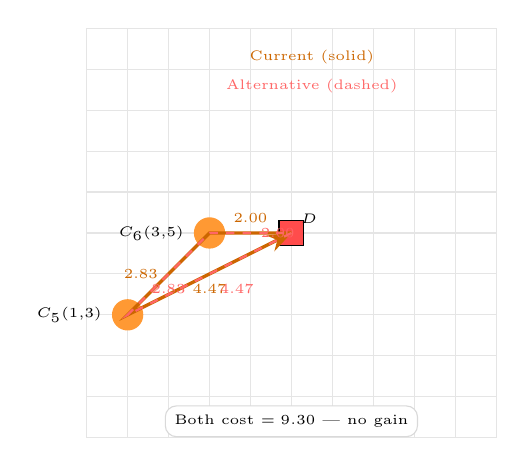
\begin{tikzpicture}[scale=0.52,>=Stealth]
  \draw[gray!20](0,0) grid (10,10);
  \node[draw,rectangle,fill=red!70,minimum size=9pt](D) at (5,5){};
  \node[font=\tiny,above right] at (5,5){$D$};
  \node[circle,fill=orange!80,inner sep=4pt,
        label=left:{\tiny $C_6(3{,}5)$}](c6) at (3,5){};
  \node[circle,fill=orange!80,inner sep=4pt,
        label=left:{\tiny $C_5(1{,}3)$}](c5) at (1,3){};
  % current route
  \draw[->,orange!80!black,very thick](5,5)
       --node[above,font=\tiny]{2.00}(3,5)
       --node[left,font=\tiny]{2.83}(1,3)
       --node[below,font=\tiny]{4.47}(5,5);
  % alternative
  \draw[red!60,dashed,thick](5,5)
       --node[below right,font=\tiny]{4.47}(1,3)
       --node[below,font=\tiny]{2.83}(3,5)
       --node[right,font=\tiny]{2.00}(5,5);
  \node[font=\tiny,orange!80!black] at (5.5,9.3){Current (solid)};
  \node[font=\tiny,red!60] at (5.5,8.6){Alternative (dashed)};
  \node[font=\tiny,fill=white,draw=gray!30,rounded corners] at (5,0.4)
       {Both cost $=9.30$ --- no gain};
\end{tikzpicture}
\end{center}
\end{columns}
\end{frame}

% Page 29 (moved): Enhanced Sweep — Inter-Route Relocate Check
\begin{frame}[shrink=5]{Enhanced Sweep --- Inter-Route Relocate Check}
\begin{columns}[T]
\column{0.50\textwidth}
\small
R3: $D\!\to\!C_4\!\to\!D$, load $=18$\\
R4: $D\!\to\!C_3\!\to\!D$, load $=15$

\vspace{0.3em}
\textbf{Try:} Move $C_4$ from R3 into R4.\\
Capacity: $15+18=33>30$ \textbf{--- Infeasible.}

\vspace{0.2em}
\textbf{Try:} Move $C_3$ from R4 into R3.\\
Capacity: $18+15=33>30$ \textbf{--- Infeasible.}

\vspace{0.2em}
\textbf{Try:} Move $C_3$ into R1 (after $C_2$).\\
R1 load: $22+15=37>30$ \textbf{--- Infeasible.}

\vspace{0.2em}
\textbf{Try:} Move $C_3$ into R2 (after $C_6$).\\
R2 load: $22+15=37>30$ \textbf{--- Infeasible.}

\vspace{0.3em}
\begin{block}{Conclusion}
\footnotesize No feasible relocate improves the solution. The 4-route result is confirmed by the enhanced solver too.
\end{block}

\column{0.46\textwidth}
\begin{center}
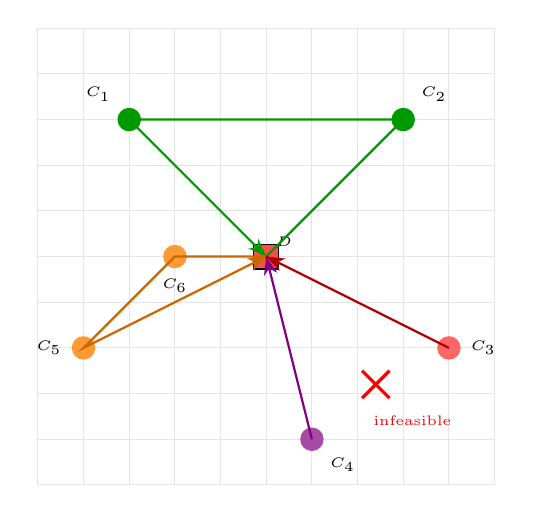
\begin{tikzpicture}[scale=0.58,>=Stealth]
  \draw[gray!20](0,0) grid (10,10);
  \node[draw,rectangle,fill=red!70,minimum size=9pt] at (5,5){};
  \node[font=\tiny,above right] at (5,5){$D$};
  \node[circle,fill=green!60!black,inner sep=3pt,
        label=above right:{\tiny $C_2$}] at (8,8){};
  \node[circle,fill=green!60!black,inner sep=3pt,
        label=above left:{\tiny $C_1$}]  at (2,8){};
  \draw[->,green!60!black,thick](5,5)--(8,8)--(2,8)--(5,5);
  \node[circle,fill=orange!80,inner sep=3pt,
        label=below:{\tiny $C_6$}] at (3,5){};
  \node[circle,fill=orange!80,inner sep=3pt,
        label=left:{\tiny $C_5$}]  at (1,3){};
  \draw[->,orange!80!black,thick](5,5)--(3,5)--(1,3)--(5,5);
  \node[circle,fill=violet!70,inner sep=3pt,
        label=below right:{\tiny $C_4$}] at (6,1){};
  \draw[->,violet,thick](5,5)--(6,1)--(5,5);
  \node[circle,fill=red!60,inner sep=3pt,
        label=right:{\tiny $C_3$}] at (9,3){};
  \draw[->,red!70!black,thick](5,5)--(9,3)--(5,5);
  % blocked arrows
  \draw[red,very thick](7.1,1.9)--(7.7,2.5);
  \draw[red,very thick](7.7,1.9)--(7.1,2.5);
  \node[font=\tiny,red] at (8.2,1.4){infeasible};
\end{tikzpicture}
\end{center}
\end{columns}
\end{frame}

% Page 30 (moved): Enhanced Sweep — Inter-Route Swap Check
\begin{frame}[shrink=5]{Enhanced Sweep --- Inter-Route Swap Check}
\begin{columns}[T]
\column{0.52\textwidth}
\small
\textbf{Try:} Swap $C_1$ (R1) $\leftrightarrow$ $C_6$ (R2).

\vspace{0.2em}
Feasibility R1: $22-10+14=26\leq30$ \checkmark\\
Feasibility R2: $22-14+10=18\leq30$ \checkmark

\vspace{0.3em}
$\Delta$ cost:
\footnotesize
\[
\text{Old: }d(C_2,C_1)+d(C_1,D)+d(D,C_6)+d(C_6,C_5)
\]
\[
= 6.00+4.24+2.00+2.83 = 15.07
\]
\[
\text{New: }d(C_2,C_6)+d(C_6,D)+d(D,C_1)+d(C_1,C_5)
\]
\[
= 5.10+2.00+4.24+7.28 = 18.62
\]
\normalsize
$\Delta = 18.62-15.07 = +3.55 > 0$ $\Rightarrow$ \textbf{Rejected.}

\vspace{0.2em}
\footnotesize All other swap pairs yield $\Delta\geq0$ --- no improvement.

\column{0.44\textwidth}
\begin{center}
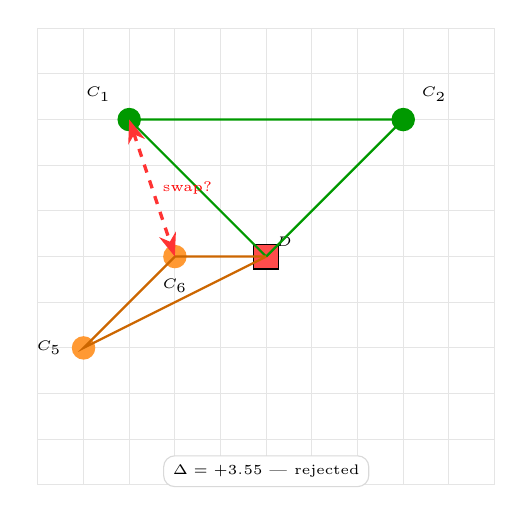
\begin{tikzpicture}[scale=0.58,>=Stealth]
  \draw[gray!20](0,0) grid (10,10);
  \node[draw,rectangle,fill=red!70,minimum size=9pt] at (5,5){};
  \node[font=\tiny,above right] at (5,5){$D$};
  \node[circle,fill=green!60!black,inner sep=3pt,
        label=above right:{\tiny $C_2$}](c2) at (8,8){};
  \node[circle,fill=green!60!black,inner sep=3pt,
        label=above left:{\tiny $C_1$}](c1) at (2,8){};
  \draw[green!60!black,thick](5,5)--(8,8)--(2,8)--(5,5);
  \node[circle,fill=orange!80,inner sep=3pt,
        label=below:{\tiny $C_6$}](c6) at (3,5){};
  \node[circle,fill=orange!80,inner sep=3pt,
        label=left:{\tiny $C_5$}](c5) at (1,3){};
  \draw[orange!80!black,thick](5,5)--(3,5)--(1,3)--(5,5);
  \draw[<->,red!80,dashed,very thick](2,8)
       --node[right,font=\tiny,red]{swap?}(3,5);
  \node[font=\tiny,fill=white,draw=gray!30,rounded corners] at (5,0.3)
       {$\Delta=+3.55$ --- rejected};
\end{tikzpicture}
\end{center}
\end{columns}
\end{frame}

% ── Or-opt ──────────────────────────────────────────────────────────────
\begin{frame}[fragile,shrink=12]{Or-opt: Moving Chains of Customers}

\begin{columns}[T]

\column{0.54\textwidth}
\begin{block}{\texttt{or\_opt(route, nodes, length)}}
\begin{lstlisting}
def or_opt(route, nodes, length):
    imp = True
    while imp:
        imp = False
        n = len(route)
        for i in range(1, n-length):
            e = i + length - 1
            rem_gain = (
              dist(nodes[route[i-1]],
                   nodes[route[i]])
            + dist(nodes[route[e]],
                   nodes[route[e+1]])
            - dist(nodes[route[i-1]],
                   nodes[route[e+1]]))
            for j in range(n-1):
                # try forward & reversed
                # insertion after j
                # if gain > 1e-9: move
                ...
    return route
\end{lstlisting}
\end{block}

\column{0.42\textwidth}
\small
\textbf{Concept:} Remove a chain of \texttt{length} consecutive customers and re-insert it at the best position (forward or reversed).

\vspace{0.4em}
\textbf{Gain calculation:}
\[
  g_{\text{rem}} = d_{i-1,i} + d_{e,e+1} - d_{i-1,e+1}
\]
\[
  g_{\text{ins}} = d_{j,i} + d_{e,j+1} - d_{j,j+1}
\]
Move if $g_{\text{rem}} - g_{\text{ins}} > \epsilon$.

\vspace{0.4em}
\textbf{Called with lengths 1, 2, 3:}\\
\footnotesize
\texttt{or\_opt(r, nodes, 1)} — relocate\\
\texttt{or\_opt(r, nodes, 2)} — move pair\\
\texttt{or\_opt(r, nodes, 3)} — move triple
\end{columns}

\end{frame}

% ── Intra-LS ────────────────────────────────────────────────────────────
\begin{frame}[fragile]{Intra-Route Local Search Pipeline}

\begin{columns}[T]

\column{0.5\textwidth}
\begin{block}{\texttt{intra\_ls(route, nodes)}}
\begin{lstlisting}
def intra_ls(route, nodes):
    prev = float("inf")
    while True:
        prev = route_cost(route,
                          nodes)
        route = two_opt(route,
                        nodes)
        route = or_opt(route,
                       nodes, 1)
        route = or_opt(route,
                       nodes, 2)
        route = or_opt(route,
                       nodes, 3)
        if route_cost(route, nodes)\
                >= prev - 1e-9:
            break
    return route
\end{lstlisting}
\end{block}

\column{0.46\textwidth}
\small
\textbf{Iterates until stable:}

\vspace{0.3em}
\begin{center}
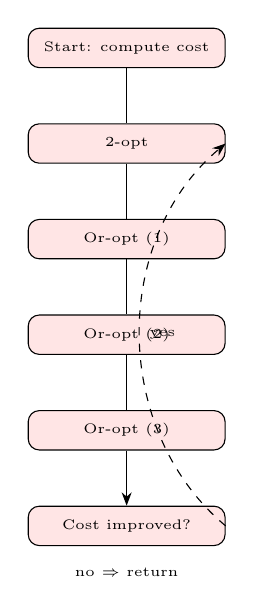
\begin{tikzpicture}[>=Stealth, node distance=0.7cm,
    b/.style={draw, rounded corners, fill=red!10,
              minimum width=2.5cm, minimum height=0.5cm,
              font=\tiny, align=center}]
  \node[b] (s) {Start: compute cost};
  \node[b] (t) [below=of s] {2-opt};
  \node[b] (o1)[below=of t] {Or-opt (1)};
  \node[b] (o2)[below=of o1]{Or-opt (2)};
  \node[b] (o3)[below=of o2]{Or-opt (3)};
  \node[b] (c) [below=of o3]{Cost improved?};
  \draw[->] (s)--(t)--(o1)--(o2)--(o3)--(c);
  \draw[->, dashed] (c.east) to[bend left=50]
        node[right,font=\tiny]{yes} (t.east);
  \node[font=\tiny, below=0.15cm of c] {no $\Rightarrow$ return};
\end{tikzpicture}
\end{center}
\end{columns}

\end{frame}

% ── Inter-route relocate ─────────────────────────────────────────────────
\begin{frame}[fragile]{Inter-Route Relocate}

\begin{columns}[T]

\column{0.54\textwidth}
\begin{block}{\texttt{inter\_relocate(routes, nodes, cap)}}
\begin{lstlisting}
for a in range(R):
  pi = 1
  while pi + 1 < len(routes[a]):
    cu = routes[a][pi]
    rem_gain = (
      dist(nodes[routes[a][pi-1]],
           nodes[cu])
    + dist(nodes[cu],
           nodes[routes[a][pi+1]])
    - dist(nodes[routes[a][pi-1]],
           nodes[routes[a][pi+1]]))
    best_gain = 1e-9
    for b in range(R):
      if b == a: continue
      if (route_demand(routes[b])
          + nodes[cu].demand > cap):
        continue
      # find best insertion pos
      ...
    if best_b != -1:
      routes[a].pop(pi)
      routes[best_b].insert(
          best_pos, cu)
\end{lstlisting}
\end{block}

\column{0.42\textwidth}
\small
\textbf{Goal:} Move a single customer $c_u$ from route $a$ to the best feasible position in any other route $b$.

\vspace{0.3em}
\textbf{Feasibility check:}
\[
  \sum_{i \in b} d_i + d_{c_u} \leq Q
\]

\vspace{0.3em}
\textbf{Net gain:}
\[
  \Delta = g_{\text{remove}} - g_{\text{insert}}
\]
Move if $\Delta > 10^{-9}$.

\vspace{0.3em}
\footnotesize Empty routes (depot $\to$ depot only) are automatically pruned after each pass.
\end{columns}

\end{frame}

% ── Inter-route swap ─────────────────────────────────────────────────────
\begin{frame}[fragile]{Inter-Route Swap}

\begin{columns}[T]

\column{0.54\textwidth}
\begin{block}{\texttt{inter\_swap(routes, nodes, cap)}}
\begin{lstlisting}
for a in range(R):
  for pi in range(1,
        len(routes[a])-1):
    for b in range(a+1, R):
      for qi in range(1,
            len(routes[b])-1):
        cu = routes[a][pi]
        cv = routes[b][qi]
        # check both capacity
        # constraints
        ...
        delta = (
          dist(...cv...) +
          dist(...cv...) +
          dist(...cu...) +
          dist(...cu...)
          - dist(...cu...) * 2
          - dist(...cv...) * 2)
        if delta < -1e-9:
          routes[a][pi] = cv
          routes[b][qi] = cu
\end{lstlisting}
\end{block}

\column{0.42\textwidth}
\small
\textbf{Goal:} Swap customer $c_u \in$ route $a$ with customer $c_v \in$ route $b$.

\vspace{0.3em}
\textbf{Feasibility (both routes):}
\[
  \Sigma_a - d_{c_u} + d_{c_v} \leq Q
\]
\[
  \Sigma_b - d_{c_v} + d_{c_u} \leq Q
\]

\vspace{0.3em}
\textbf{$\Delta$ cost} (sum of 4 new edges minus 4 old edges). Accept if $\Delta < -10^{-9}$.

\vspace{0.3em}
\textbf{Complexity:} $O(R^2 \cdot n^2)$ per pass; at most 20 passes.
\end{columns}

\end{frame}

% ── Multi-start ──────────────────────────────────────────────────────────
\begin{frame}[fragile,shrink=10]{Multi-Start Sweep ($K=8$)}

\begin{columns}[T]

\column{0.54\textwidth}
\begin{block}{\texttt{solve(nodes, dimension, capacity)}}
\begin{lstlisting}
K = 8
best_routes = None
best_cost   = float("inf")

for k in range(K):
    start_angle = k*(2*pi/K)

    # rotate customer order
    order = []
    for c in customers:
        a = c.angle - start_angle
        if a < 0: a += 2*pi
        order.append((a, c.id))
    order.sort()

    # cluster + NN + intra-LS
    ...
    c = total_cost(routes, nodes)
    if c < best_cost:
        best_cost   = c
        best_routes = deepcopy(routes)

# Inter-route improvement
for _ in range(20):
    r1 = inter_relocate(...)
    r2 = inter_swap(...)
    if not r1 and not r2: break
    # quick 2-opt + or-opt touchup
\end{lstlisting}
\end{block}

\column{0.42\textwidth}
\small
\textbf{Starting angles:}
\[
  \alpha_k = \frac{2\pi k}{8}, \quad k = 0,1,\ldots,7
\]

Each start produces a different clustering. The best solution (lowest total cost) is kept.

\vspace{0.4em}
\begin{center}
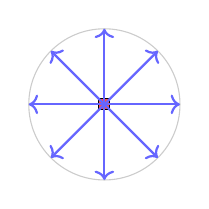
\begin{tikzpicture}[scale=0.8]
  \draw[gray!40] (0,0) circle(1.2);
  \node[draw,rectangle,fill=red!70,inner sep=2pt] at (0,0) {};
  \draw[->,blue!60,thick] (0,0) -- (0:1.2);
  \draw[->,blue!60,thick] (0,0) -- (45:1.2);
  \draw[->,blue!60,thick] (0,0) -- (90:1.2);
  \draw[->,blue!60,thick] (0,0) -- (135:1.2);
  \draw[->,blue!60,thick] (0,0) -- (180:1.2);
  \draw[->,blue!60,thick] (0,0) -- (225:1.2);
  \draw[->,blue!60,thick] (0,0) -- (270:1.2);
  \draw[->,blue!60,thick] (0,0) -- (315:1.2);
\end{tikzpicture}\\
\footnotesize 8 sweep directions
\end{center}
\end{columns}

\end{frame}

% ======================================================================
\section{Worked Example Simulation}
% ======================================================================

% ── Slide: final comparison ─────────────────────────────────────────────
\begin{frame}[shrink=8]{Worked Example --- Final Results}
\begin{block}{Instance: 6 customers, $Q=30$, Depot $(5,5)$}
\centering
\begin{tabular}{lccc}
\toprule
\textbf{Algorithm} & \textbf{Routes} & \textbf{Total Cost} & \textbf{Note} \\
\midrule
Gillett \& Miller & 4 & 40.03 & Single start \\
Enhanced Sweep    & 4 & 40.03 & Best of 8 starts (identical here) \\
\bottomrule
\end{tabular}
\end{block}
\vspace{0.3em}
\begin{columns}[T]
\column{0.50\textwidth}
\small\textbf{Route breakdown:}
\begin{itemize}
  \item R1: $D\!\to\!C_2\!\to\!C_1\!\to\!D$, load $22$, cost $14.48$
  \item R2: $D\!\to\!C_6\!\to\!C_5\!\to\!D$, load $22$, cost $9.30$
  \item R3: $D\!\to\!C_4\!\to\!D$, load $18$, cost $8.25$
  \item R4: $D\!\to\!C_3\!\to\!D$, load $15$, cost $8.00$
\end{itemize}
\column{0.46\textwidth}
\small\textbf{Key observations:}
\begin{itemize}
  \item $C_3+C_4$: $15+18=33>30$ --- cannot share a vehicle.
  \item 4 routes are structurally unavoidable for $Q=30$.
  \item Enhanced confirms via relocate/swap that no improvement exists.
  \item On larger instances the multi-start and inter-route operators give measurable gains.
\end{itemize}
\end{columns}
\end{frame}

% ── Algorithm comparison ─────────────────────────────────────────────────
\begin{frame}{Algorithm Comparison: Gillett vs.\ Enhanced}

\begin{center}
\resizebox{0.96\textwidth}{!}{%
\begin{tabular}{lll}
\toprule
\textbf{Feature} & \textbf{Gillett \& Miller} & \textbf{Enhanced Sweep} \\
\midrule
Starting angles    & 1 (fixed at 0)         & 8 (evenly spaced) \\
Intra-route LS     & 2-opt only             & 2-opt + Or-opt (1/2/3) \\
Inter-route LS     & None                   & Relocate + Swap (20 passes) \\
Post-move touch-up & None                   & 2-opt + Or-opt (1) \\
Solution quality   & Good                   & Better (typically) \\
Runtime            & Very fast              & Moderate \\
Output files       & \texttt{\_sweep\_gillett.*} & \texttt{\_enhanced.*} \\
\bottomrule
\end{tabular}
}
\end{center}

\vspace{0.5em}

\begin{block}{Key Insight}
The $K$-start approach hedges against bad sweep angles.
The inter-route operators allow customers to ``migrate'' between
routes, fixing imbalances that no intra-route method can resolve.
\end{block}

\end{frame}

% ======================================================================
\section{Comparison Extractor (\texttt{extract.py})}
% ======================================================================

% ── Sample output (REPLACED with actual comparison_results.txt data) ────
\begin{frame}[fragile]{Sample Output: \texttt{comparison\_results.txt}}

\begin{lstlisting}[language={},numbers=none,basicstyle=\ttfamily\fontsize{5}{6}\selectfont]
+------------------------+--------------+----------------+----------------+----------+----------+
| Instance               | Optimal(.sol)| Gillett Sweep  | Enhanced       | GapGilt% | GapEnh%  |
+------------------------+--------------+----------------+----------------+----------+----------+
| A-n32-k5               | 784.00       | 885.04         | 885.04         | 12.89    | 12.89    |
| A-n33-k5               | 661.00       | 792.40         | 698.30         | 19.88    |  5.64    |
| A-n33-k6               | 742.00       | 875.32         | 751.65         | 17.97    |  1.30    |
| A-n34-k5               | 778.00       | 868.75         | 786.44         | 11.66    |  1.08    |
| A-n36-k5               | 799.00       | 950.36         | 874.86         | 18.94    |  9.49    |
| A-n37-k5               | 669.00       | 841.56         | 737.31         | 25.79    | 10.21    |
| A-n37-k6               | 949.00       | 1136.51        | 1038.62        | 19.76    |  9.44    |
| A-n38-k5               | 730.00       | 880.83         | 776.05         | 20.66    |  6.31    |
| A-n39-k5               | 822.00       | 1014.97        | 881.35         | 23.48    |  7.22    |
| A-n39-k6               | 831.00       | 991.54         | 896.92         | 19.32    |  7.93    |
| A-n44-k6               | 937.00       | 1166.04        | 1055.96        | 24.44    | 12.70    |
| A-n45-k6               | 944.00       | 1116.09        | 1049.70        | 18.23    | 11.20    |
| A-n45-k7               | 1146.00      | 1342.89        | 1306.53        | 17.18    | 14.01    |
| A-n46-k7               | 914.00       | 1039.92        | 961.04         | 13.78    |  5.15    |
| A-n48-k7               | 1073.00      | 1155.59        | 1147.35        |  7.70    |  6.93    |
| A-n53-k7               | 1010.00      | 1176.36        | 1088.12        | 16.47    |  7.73    |
| A-n54-k7               | 1167.00      | 1368.72        | 1320.84        | 17.29    | 13.18    |
| A-n55-k9               | 1073.00      | 1204.19        | 1172.99        | 12.23    |  9.32    |
| A-n60-k9               | 1354.00      | 1680.92        | 1450.92        | 24.14    |  7.16    |
| A-n61-k9               | 1034.00      | 1226.47        | 1093.82        | 18.61    |  5.79    |
| A-n62-k8               | 1288.00      | 1624.06        | 1386.20        | 26.09    |  7.62    |
| A-n63-k10              | 1314.00      | 1555.07        | 1409.67        | 18.35    |  7.28    |
| A-n63-k9               | 1616.00      | 1828.05        | 1789.02        | 13.12    | 10.71    |
| A-n64-k9               | 1401.00      | 1599.79        | 1508.46        | 14.19    |  7.67    |
| A-n65-k9               | 1174.00      | 1373.00        | 1286.49        | 16.95    |  9.58    |
| A-n69-k9               | 1159.00      | 1271.82        | 1255.55        |  9.73    |  8.33    |
| A-n80-k10              | 1763.00      | 2142.94        | 1981.53        | 21.55    | 12.40    |
+------------------------+--------------+----------------+----------------+----------+----------+
| AVERAGE                | 1041.93      | 1226.27        | 1132.99        | 17.69    |  8.74    |
+------------------------+--------------+----------------+----------------+----------+----------+
  Enhanced wins: 26 instance(s)   Gillett wins: 0   Tied: 1   Total: 27
\end{lstlisting}

\end{frame}

% ── Route plot: Gillett A-n80-k10 ───────────────────────────────────────
\begin{frame}{Route Plot: A-n80-k10 — Gillett Sweep}
\begin{center}
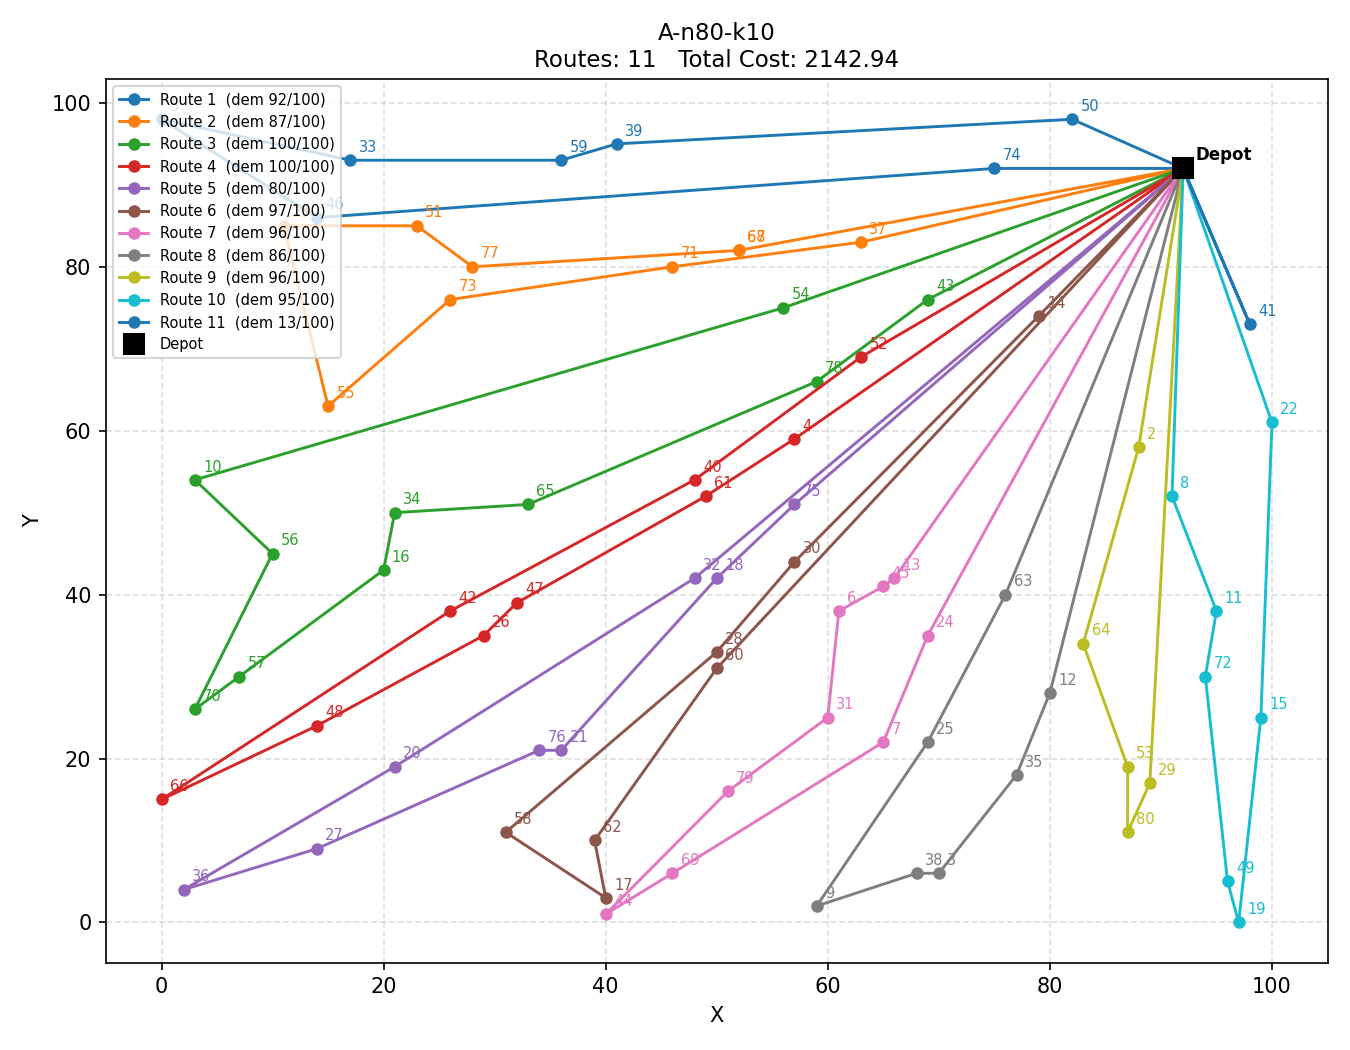
\includegraphics[width=0.85\textwidth]{A-n80-k10_sweep_gillett.png}
\end{center}
\end{frame}

% ── Route plot: Enhanced A-n80-k10 ──────────────────────────────────────
\begin{frame}{Route Plot: A-n80-k10 — Enhanced Sweep}
\begin{center}
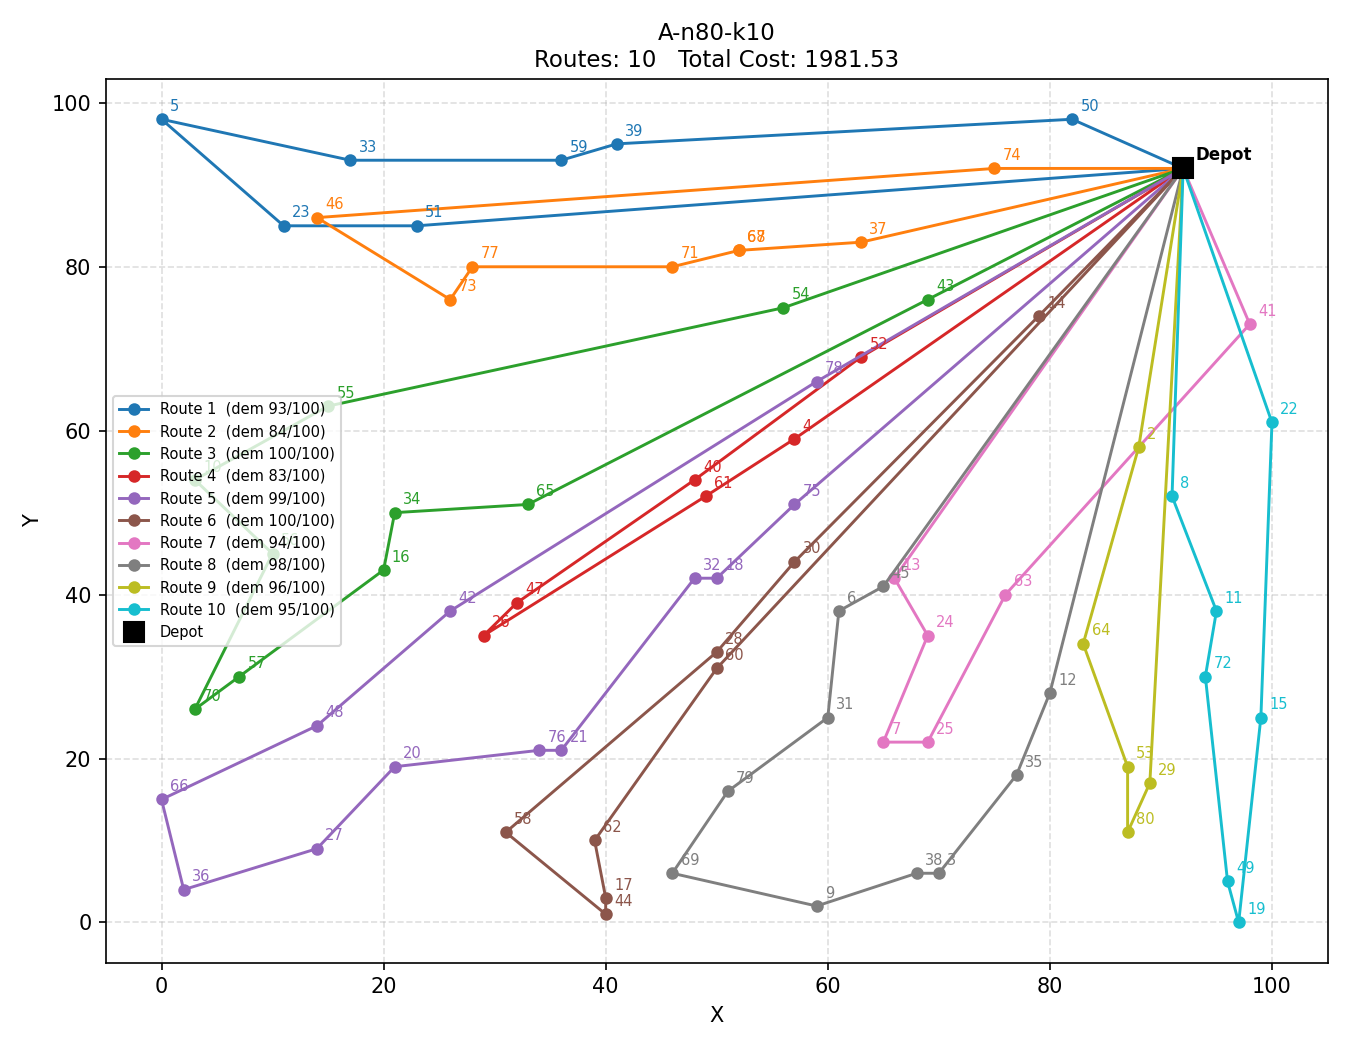
\includegraphics[width=0.85\textwidth]{A-n80-k10_enhanced.png}
\end{center}
\end{frame}



% ======================================================================
\section{Implementation Details}
% ======================================================================

% ── Complexity summary ────────────────────────────────────────────────────
\begin{frame}{Complexity Summary}

\begin{center}
\resizebox{0.95\textwidth}{!}{%
\begin{tabular}{llll}
\toprule
\textbf{Operation} & \textbf{Complexity} & \textbf{Used in} & \textbf{Notes} \\
\midrule
Polar angle sort      & $O(n \log n)$         & Both solvers     & Once per start \\
Greedy clustering     & $O(n)$                & Both solvers     & Linear scan \\
Nearest-neighbour     & $O(|C|^2)$ per cluster & Both solvers    & $\sum|C|=n$ \\
2-opt                 & $O(n^2)$ per pass     & Both solvers     & Repeats until stable \\
Or-opt (len $\ell$)   & $O(n^2)$ per pass     & Enhanced         & $\ell \in \{1,2,3\}$ \\
Inter-route relocate  & $O(R \cdot n^2)$ per pass & Enhanced    & Up to 20 passes \\
Inter-route swap      & $O(R^2 \cdot n^2)$ per pass & Enhanced  & Up to 20 passes \\
Multi-start           & $\times K = 8$        & Enhanced         & Best of 8 kept \\
\bottomrule
\end{tabular}
}
\end{center}

\vspace{0.4em}
\begin{center}
\small $n$ = number of customers, $R$ = number of routes, $C$ = cluster
\end{center}

\end{frame}

%==================================================================
%
%     Add slides for metaheuristics below:
%
%==================================================================

% =============================================================================
\section{Original Genetic Algorithm}
% =============================================================================

\begin{frame}{Genetic Algorithm -- Background}
  Genetic Algorithms (GAs) are population-based evolutionary search methods
  inspired by natural selection \cite{holland1975adaptation, goldberg1989genetic}.
  \vspace{6pt}

  \begin{columns}
    \column{0.5\textwidth}
    \textbf{Why GA for CVRP?}
    \begin{itemize}
      \item Can escape local optima via population diversity
      \item Flexible representation for combinatorial problems
      \item Easily extended with domain-specific operators
      \item No gradient information required
    \end{itemize}

    \column{0.48\textwidth}
    \textbf{Giant-tour representation}
    \begin{itemize}
      \item Chromosome = permutation of all $n$ customer IDs
      \item Decoded by greedy split: scan the tour and start a new route
            whenever the next customer would exceed $C$
      \item Simple, always feasible, no repair needed
    \end{itemize}
  \end{columns}
\end{frame}

\begin{frame}{Original GA -- Algorithm}
  \begin{algorithm}[H]
  \caption{Original Genetic Algorithm for CVRP}
  \begin{algorithmic}[1]
    \State $P \leftarrow$ \textbf{RandomPopulation}$(N_{\text{pop}})$
    \For{$g = 1$ \textbf{to} $G_{\max}$}
      \State Evaluate fitness: $f(c) = \text{TotalDist}(\text{Decode}(c))$ for all $c \in P$
      \State $P' \leftarrow$ \textbf{Elites}$(P,\, e)$  \Comment{keep top $e$ unchanged}
      \While{$|P'| < N_{\text{pop}}$}
        \State $p_1, p_2 \leftarrow$ \textbf{TournamentSelect}$(P,\, k=3)$
        \State $c_1, c_2 \leftarrow$ \textbf{OX1Crossover}$(p_1, p_2)$ with prob.\ $p_c$
        \State $c_1 \leftarrow$ \textbf{Mutate}$(c_1)$;\; $c_2 \leftarrow$ \textbf{Mutate}$(c_2)$
        \State Append $c_1, c_2$ to $P'$
      \EndWhile
      \State $P \leftarrow P'$
    \EndFor
    \State \Return best chromosome seen
  \end{algorithmic}
  \end{algorithm}
\end{frame}

\begin{frame}{Original GA -- Operators}
  \begin{columns}
    \column{0.48\textwidth}
    \textbf{Order Crossover (OX1)} \cite{davis1985applying}
    \begin{enumerate}
      \item Choose a random segment $[a, b]$ from parent $P_1$
      \item Copy $P_1[a\ldots b]$ into the child at positions $a\ldots b$
      \item Fill remaining positions from $P_2$ in order, wrapping around
    \end{enumerate}
    Preserves the relative ordering of customer visits.

    \vspace{8pt}
    \textbf{Mutation (50/50 choice)}
    \begin{itemize}
      \item \emph{Swap}: exchange two random positions
      \item \emph{Inversion}: reverse a random sub-segment
    \end{itemize}

    \column{0.48\textwidth}
    \textbf{Parameters used}
    \begin{center}
    \begin{tabular}{ll}
      \toprule
      Parameter & Value \\
      \midrule
      Population size     & 100  \\
      Generations         & 300  \\
      Crossover rate      & 0.9  \\
      Mutation rate       & 0.2  \\
      Tournament size     & 3    \\
      Elite size          & 5    \\
      Random seed         & 42   \\
      \bottomrule
    \end{tabular}
    \end{center}
  \end{columns}
\end{frame}

% =============================================================================
\section{Proposed Modifications (Improved GA)}
% =============================================================================

\begin{frame}{Proposed Modifications -- Overview}
  Three targeted improvements are proposed to address the main weaknesses
  of the original GA:

  \vspace{6pt}
  \begin{enumerate}
    \setlength{\itemsep}{8pt}
    \item \textbf{Nearest-Neighbour Seeded Initialisation}\\
          \textit{Problem solved}: random initialisation produces very poor
          starting tours; the GA wastes generations escaping terrible solutions.

    \item \textbf{Intra-route 2-opt Local Search}\\
          \textit{Problem solved}: crossover and mutation alone cannot reliably
          eliminate edge crossings inside a single route; local search is
          essential to reach high-quality routes.

    \item \textbf{Adaptive Mutation Rate}\\
          \textit{Problem solved}: a fixed mutation rate is either too low
          (population stagnates in a local optimum) or too high (good
          solutions are destroyed).
  \end{enumerate}
\end{frame}

\begin{frame}{Modification 1 -- Nearest-Neighbour Seeded Initialisation}
  \begin{block}{Idea}
    Seed 20\% of the initial population with greedy nearest-neighbour tours,
    each starting from a different customer.  The remaining 80\% stay random.
  \end{block}

  \vspace{4pt}
  \textbf{Nearest-neighbour heuristic}:
  \begin{enumerate}
    \item Start at a given customer
    \item Repeatedly move to the closest unvisited customer
    \item Stop when all customers are added
  \end{enumerate}

  \vspace{4pt}
  \textbf{Reasoning}:
  \begin{itemize}
    \item NN tours are typically 20--30\% above optimal, far better than random
    \item Provides the GA with diverse but high-quality starting seeds
    \item Retaining 80\% random individuals preserves population diversity
    \item Particularly impactful on large instances (Golden, 200--483 nodes)
          where random initialisation converges extremely slowly
  \end{itemize}
\end{frame}

\begin{frame}{Modification 2 -- Intra-route 2-opt Local Search}
  \begin{block}{Idea}
    Every $L$ generations, apply a 2-opt improvement pass to each route
    of every newly created offspring before inserting it into the population.
  \end{block}

  \vspace{4pt}
  \textbf{2-opt}: repeatedly reverse a sub-segment $[i,\,j]$ of a route if
  doing so reduces its travel distance \cite{lin1965computer}:
  \[
    \text{remove edges } (v_{i-1}, v_i)\text{ and }(v_j, v_{j+1});
    \quad\text{add } (v_{i-1}, v_j)\text{ and }(v_i, v_{j+1})
  \]

  \vspace{4pt}
  \textbf{Reasoning}:
  \begin{itemize}
    \item OX1 crossover preserves \emph{global} customer order but disrupts
          \emph{local} route geometry, creating crossings
    \item 2-opt directly eliminates these crossings within each route
    \item Applied periodically (every $L=10$ gen) -- not every generation --
          to bound the extra computation cost
    \item Routes longer than 40 nodes skip 2-opt to prevent $O(n^2)$ blow-up
  \end{itemize}
\end{frame}

\begin{frame}{Modification 3 -- Adaptive Mutation Rate}
  \begin{block}{Idea}
    Monitor stagnation (generations without improvement).  When stagnation
    exceeds a threshold, gradually raise the mutation rate to inject
    diversity.  Reset to the base rate upon finding a new best solution.
  \end{block}

  \vspace{4pt}
  \textbf{Rule}:
  \[
    \mu =
    \begin{cases}
      \mu_{\text{base}} & \text{if stagnation} < S_{\text{limit}} \\
      \min\!\Bigl(0.8,\;\mu_{\text{base}} \times
        \bigl(1 + \tfrac{\text{stagnation}}{S_{\text{limit}}}\bigr)\Bigr)
        & \text{otherwise}
    \end{cases}
  \]

  \textbf{Parameters}: $\mu_{\text{base}} = 0.2$,\; $S_{\text{limit}} = 25$.

  \vspace{4pt}
  \textbf{Reasoning}:
  \begin{itemize}
    \item A fixed low rate is insufficient to escape plateaus; a fixed high
          rate randomly destroys good building blocks
    \item Adaptive rate raises diversity only when the population is stuck,
          then returns to a conservative rate once improvement resumes
  \end{itemize}
\end{frame}

% =============================================================================
\section{Experimental Results}
% =============================================================================

\begin{frame}{Experimental Setup}
  \begin{columns}
    \column{0.5\textwidth}
    \textbf{GA Parameters}
    \begin{center}
    \begin{tabular}{ll}
      \toprule
      Parameter & Value \\
      \midrule
      Population size     & 100  \\
      Generations         & 300  \\
      Crossover rate      & 0.9  \\
      Base mutation rate  & 0.2  \\
      Tournament size     & 3    \\
      Elite size          & 5    \\
      2-opt interval $L$  & 10   \\
      Stagnation limit    & 25   \\
      Random seed         & 42   \\
      \bottomrule
    \end{tabular}
    \end{center}

    \column{0.48\textwidth}
    \textbf{Evaluation metric}
    \[
      \text{Gap\%} = \frac{\text{found} - \text{known best}}{\text{known best}} \times 100
    \]
    \begin{itemize}
      \item Lower gap = better solution
      \item Gap = 0\% means optimal solution found
      \item Both algorithms run from the same seed for fair comparison
      \item 60 instances total across 3 datasets
    \end{itemize}
  \end{columns}
\end{frame}

\begin{frame}{Results -- Dataset A (Augerat, 27 instances)}
  \begin{center}
  \small
  % FIX: tabular spec must match 6 data columns
  \begin{tabular}{lrrrrr}
    \toprule
    Instance & Optimal & Orig GA & Gap\% & Impr GA & Gap\% \\
    \midrule
    A-n32-k5  & 784  & 924  & 17.86 & 834  & 6.38 \\
    A-n33-k5  & 661  & 736  & 11.35 & 665  & 0.61 \\
    A-n38-k5  & 730  & 902  & 23.56 & 738  & 1.10 \\
    A-n45-k6  & 944  & 1292 & 36.86 & 1010 & 7.01 \\
    A-n53-k7  & 1010 & 1556 & 54.06 & 1093 & 8.22 \\
    A-n63-k10 & 1314 & 1841 & 40.11 & 1345 & 2.36 \\
    A-n80-k10 & 1763 & 2895 & 64.21 & 1933 & 9.64 \\
    \midrule
    \textbf{Avg (27)} & & & \textbf{+36.98} & & \textbf{+6.66} \\
    \bottomrule
  \end{tabular}
  \end{center}
\end{frame}

\begin{frame}{Results -- Dataset E (Eilon, 13 instances)}
  \begin{center}
  \small
  % FIX: tabular spec must match 6 data columns
  \begin{tabular}{lrrrrr}
    \toprule
    Instance & Optimal & Orig GA & Gap\% & Impr GA & Gap\% \\
    \midrule
    E-n13-k4   & 247  & 247  & 0.00   & 247  & 0.00  \\
    E-n23-k3   & 569  & 570  & 0.18   & 569  & 0.00  \\
    E-n30-k3   & 534  & 584  & 9.36   & 541  & 1.31  \\
    E-n51-k5   & 521  & 809  & 55.28  & 551  & 5.76  \\
    E-n76-k7   & 682  & 1213 & 77.86  & 786  & 15.25 \\
    E-n101-k8  & 815  & 1650 & 102.45 & 928  & 13.87 \\
    E-n101-k14 & 1067 & 1984 & 85.94  & 1256 & 17.71 \\
    \midrule
    \textbf{Avg (13)} & & & \textbf{+47.33} & & \textbf{+10.37} \\
    \bottomrule
  \end{tabular}
  \end{center}
\end{frame}

\begin{frame}{Results -- Dataset Golden (20 large instances)}
  \begin{center}
  \small
  % FIX: tabular spec must match 6 data columns
  \begin{tabular}{lrrrrr}
    \toprule
    Instance   & Optimal  & Orig GA & Gap\%  & Impr GA & Gap\%  \\
    \midrule
    Golden\_1  & 5623.47  & 22239   & 295.45 & 5809    & 3.30   \\
    Golden\_10 &  735.43  &  3443   & 368.17 &  752    & 2.25   \\
    Golden\_11 &  911.98  &  4847   & 431.47 &  908    & $-$0.44 \\
    Golden\_12 & 1100.67  &  6831   & 520.63 & 1118    & 1.57   \\
    Golden\_13 &  857.19  &  3054   & 256.31 &  955    & 11.41  \\
    Golden\_17 &  707.76  &  2323   & 228.24 &  822    & 16.14  \\
    Golden\_9  &  579.70  &  2228   & 284.35 &  554    & $-$4.43 \\
    \midrule
    \textbf{Avg (20)} & & & \textbf{+373.22} & & \textbf{+11.55} \\
    \bottomrule
  \end{tabular}
  \end{center}
  \vspace{2pt}
  \textit{\small Negative gaps: Improved GA found solutions better than the listed known best.}
\end{frame}

\begin{frame}{Summary of Results}
  \small
  \begin{center}
  \begin{tabular}{lcccc}
    \toprule
    Dataset & \multicolumn{2}{c}{Avg Gap\% $\downarrow$} & \multicolumn{2}{c}{Avg Time (s)} \\
    \cmidrule(lr){2-3}\cmidrule(lr){4-5}
    & Orig. GA & Imp. GA & Orig. GA & Imp. GA \\
    \midrule
    A (27 inst.)      & 36.98  & 6.66   & 0.5  & 1.2  \\
    E (13 inst.)      & 47.33  & 10.37  & 0.8  & 4.0  \\
    Golden (20 inst.) & 373.22 & 11.55  & 3.0  & 98.0 \\
    \midrule
    \textbf{Overall (60)} & \textbf{151.30} & \textbf{9.09} & & \\
    \bottomrule
  \end{tabular}
  \end{center}
  \vspace{4pt}
  \begin{itemize}
    \item Improved GA is \textbf{16.6$\times$ closer to optimal} on average
    \item Largest gain on Golden (large instances): random init completely fails; NN + 2-opt brings gap from $>$370\% down to $\sim$11\%
    \item Small E instances (n $<$ 30): both algorithms find near-optimal
    \item Trade-off: Improved GA is $\sim$2.5$\times$ slower on average
  \end{itemize}
\end{frame}

% \begin{frame}{Route Visualisation -- Example}
%   \begin{columns}
%     \column{0.49\textwidth}
%     \textbf{Original GA} -- A-n32-k5 (cost = 924)
%     \begin{center}
%       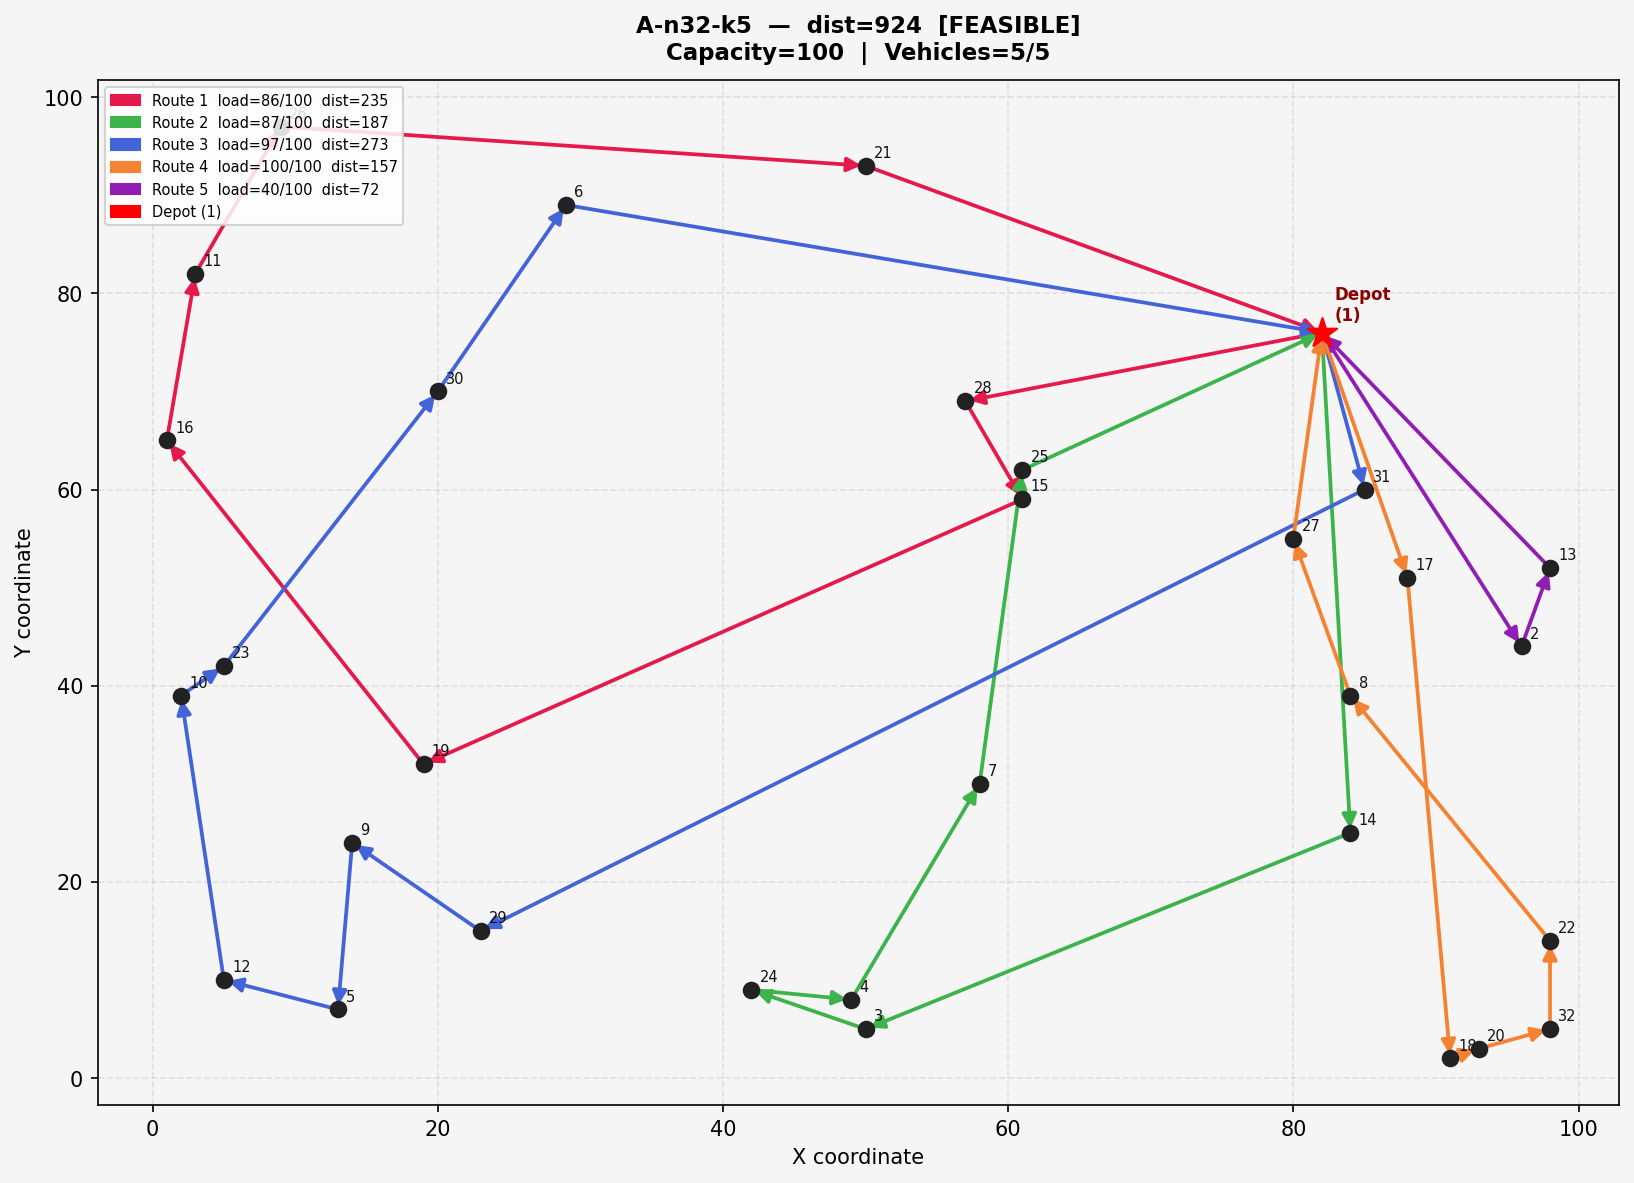
\includegraphics[width=\linewidth]{originalga_A-n32-k5_plot.png}
%     \end{center}

%     \column{0.49\textwidth}
%     \textbf{Improved GA} -- A-n32-k5 (cost = 834)
%     \begin{center}
%       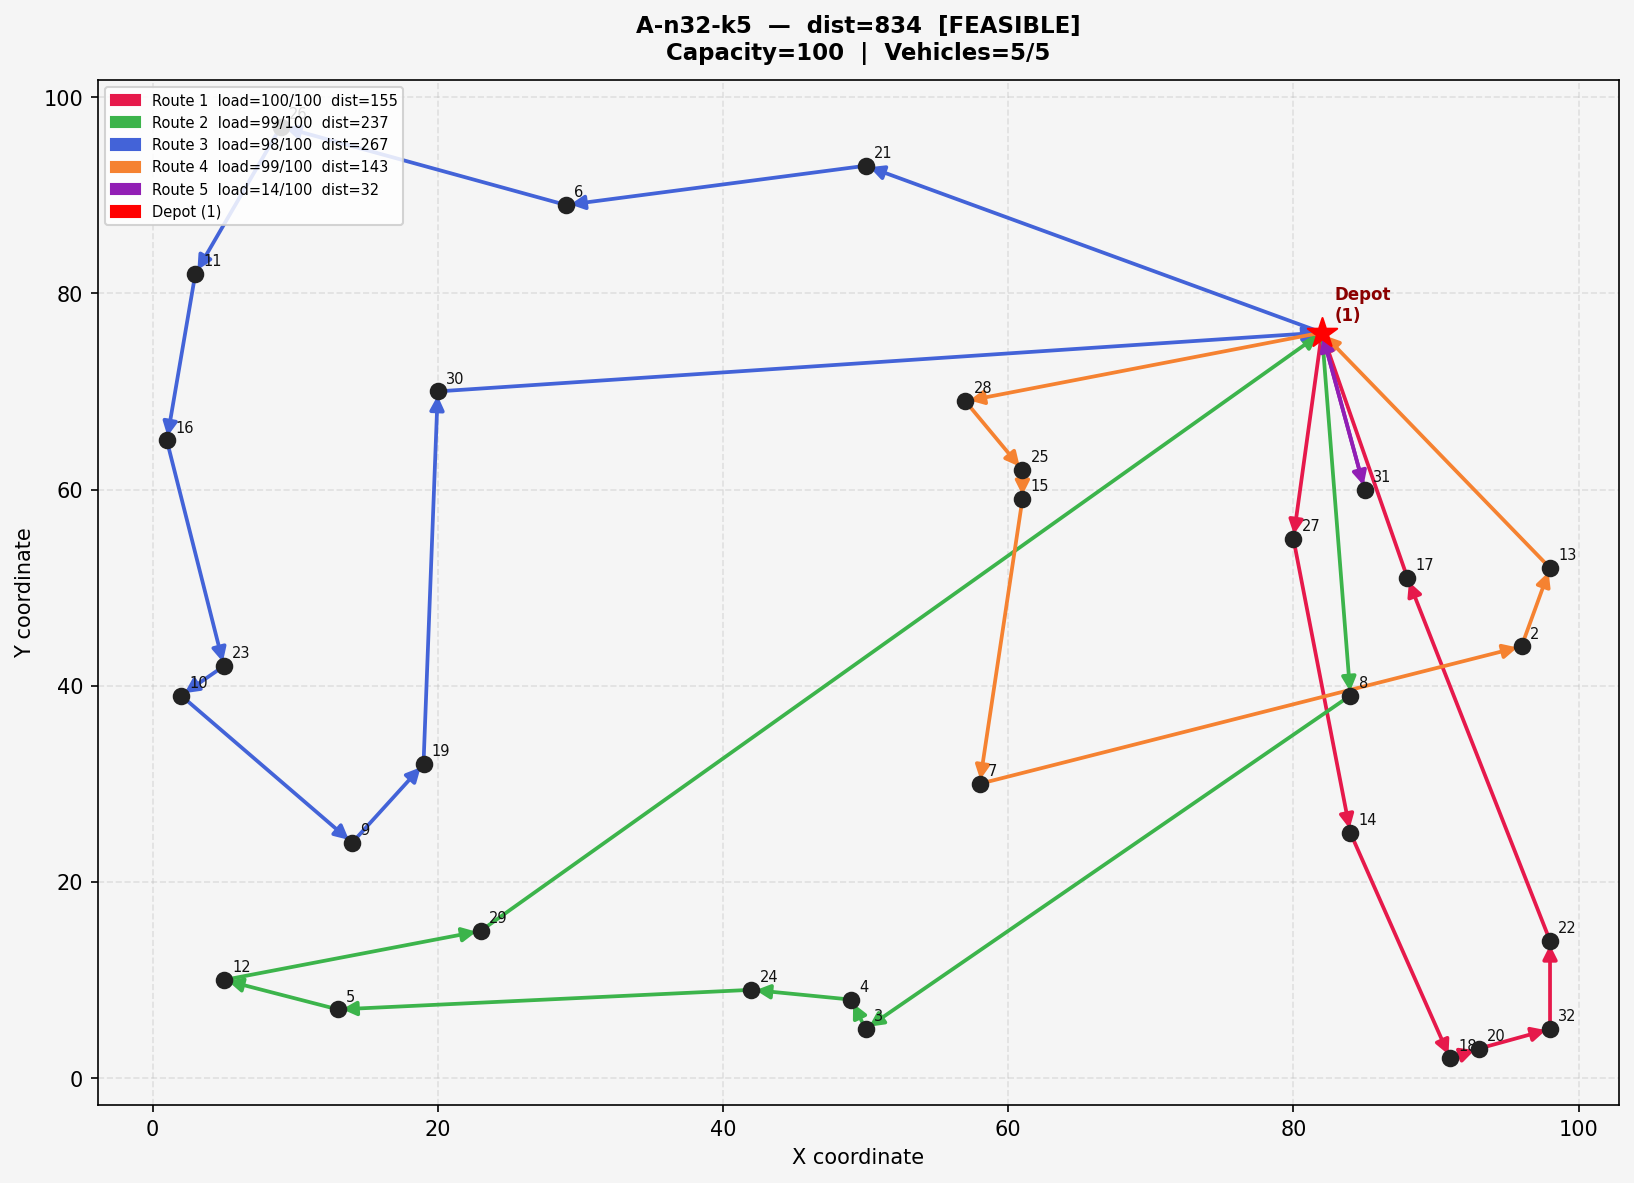
\includegraphics[width=\linewidth]{improvedga_A-n32-k5_plot.png}
%     \end{center}
%   \end{columns}
%   \vspace{4pt}
%   \textit{Optimal = 784. Improved GA gap: 6.4\% vs Original GA gap: 17.9\%.
%           The 2-opt local search visibly eliminates route crossings.}
% \end{frame}

\begin{frame}{Route Visualisation -- Example}
  \begin{columns}
    \column{0.49\textwidth}
    \textbf{Original GA} -- A-n80-k10 (cost = 2895)
    \begin{center}
      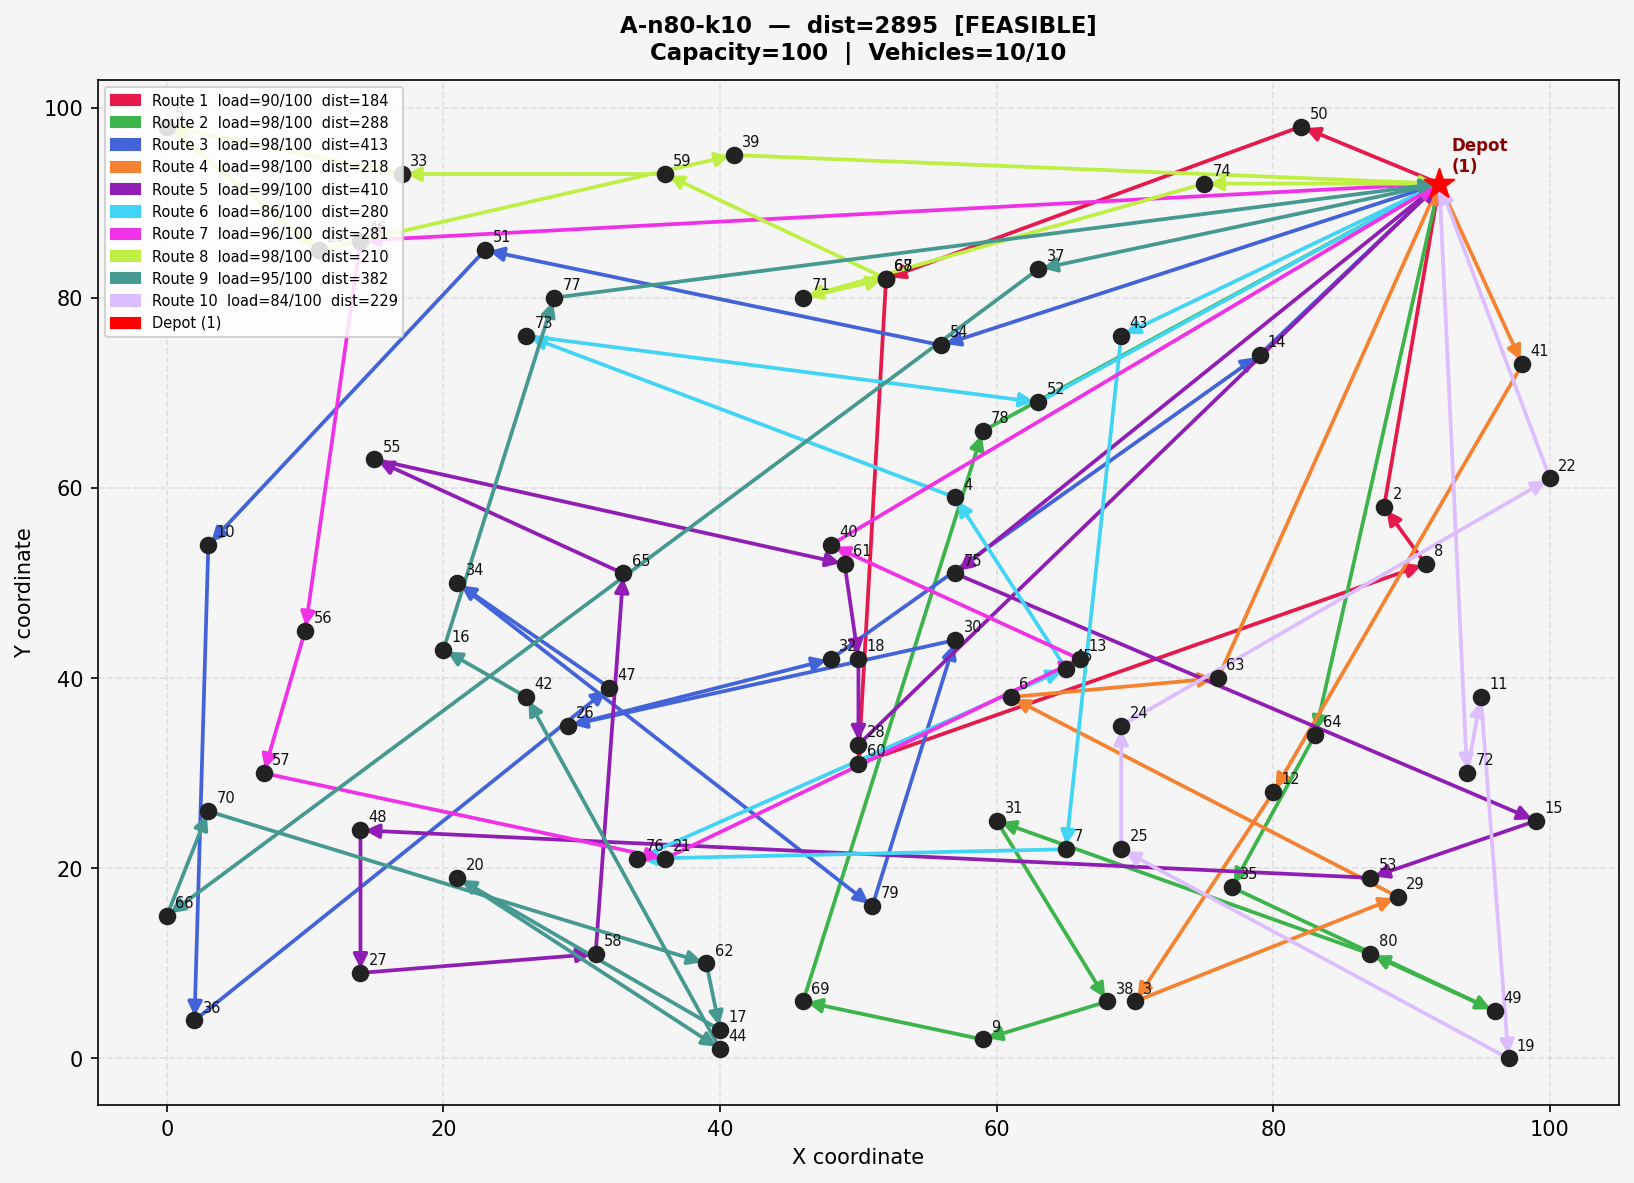
\includegraphics[width=\linewidth]{originalga_A-n80-k10_plot.png}
    \end{center}

    \column{0.49\textwidth}
    \textbf{Improved GA} -- A-n80-k10 (cost = 1933)
    \begin{center}
      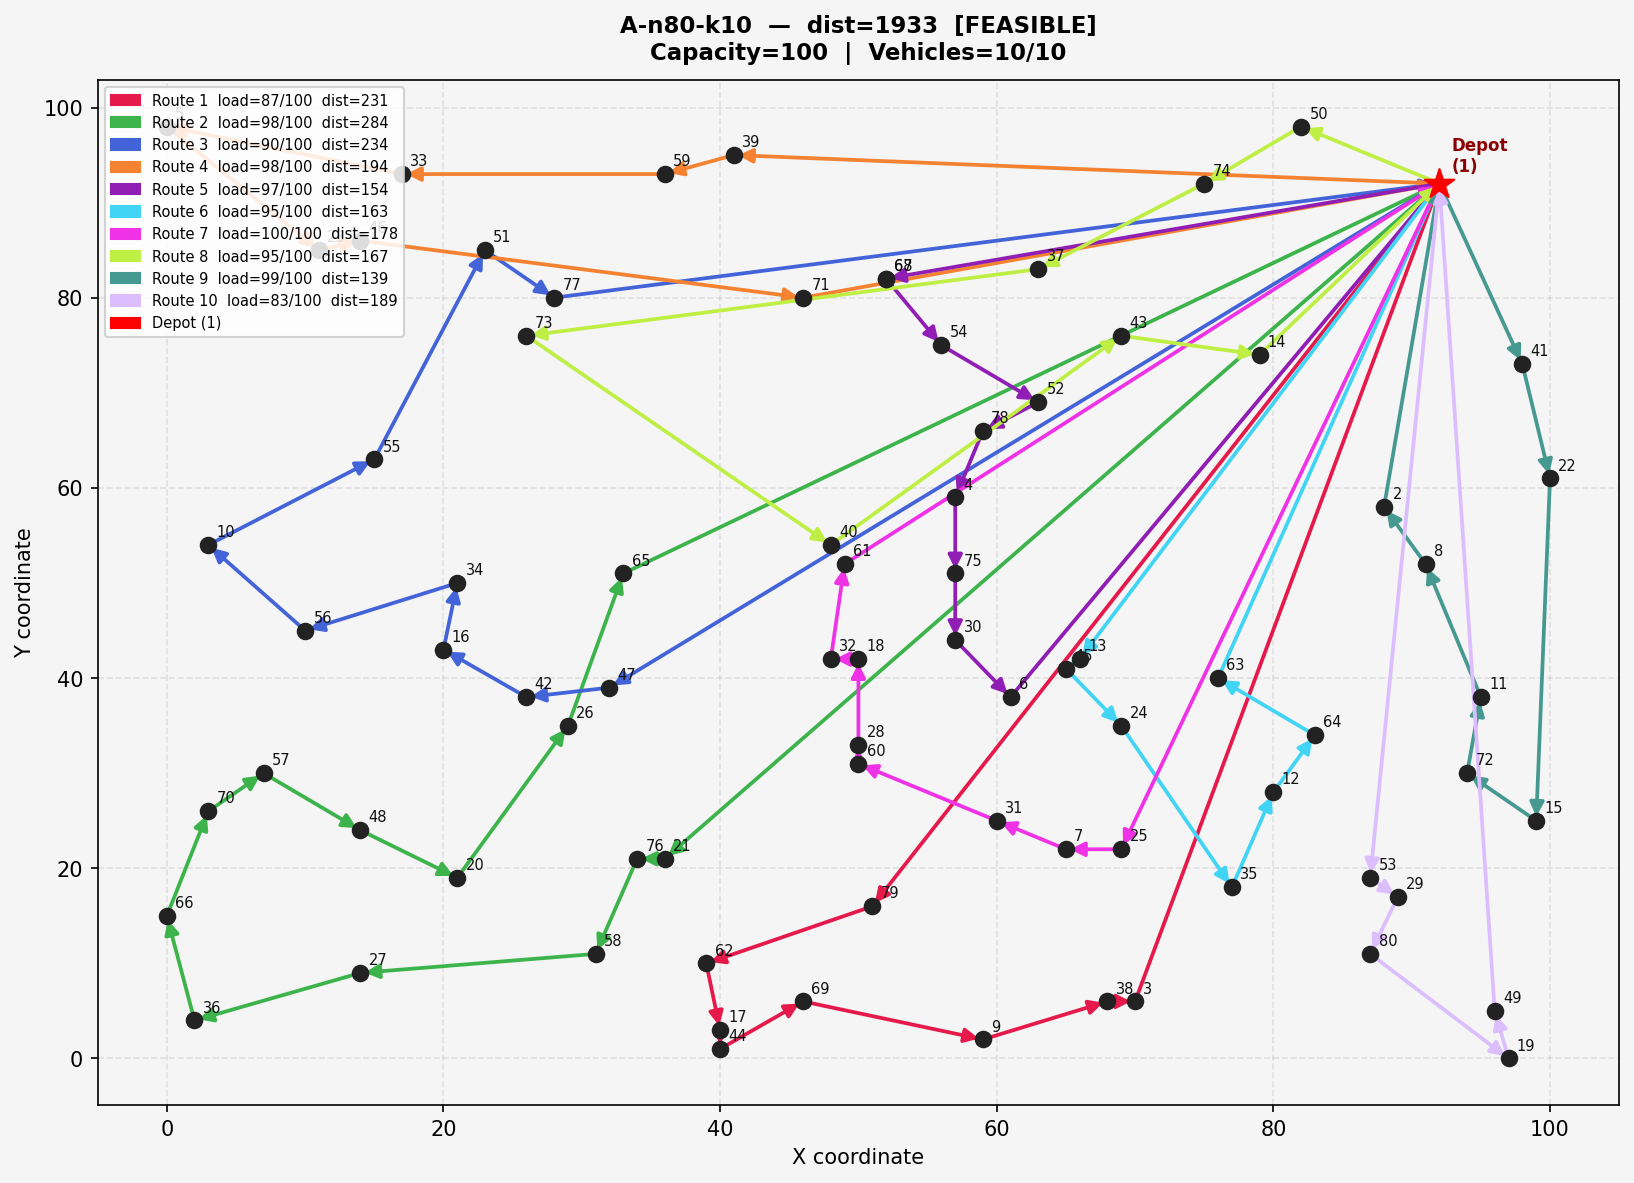
\includegraphics[width=\linewidth]{improvedga_A-n80-k10_plot.png}
    \end{center}
  \end{columns}
  \vspace{4pt}
  \textit{Optimal = 1763. Improved GA gap: 9.64\% vs Original GA gap: 64.21\%.
          The 2-opt local search visibly eliminates route crossings.}
\end{frame}

% =============================================================================
\section{Discussion \& Conclusion}
% =============================================================================

\begin{frame}{Discussion -- Impact of Each Modification}
  \begin{center}
  \begin{tabular}{lp{6.5cm}c}
    \toprule
    Modification & Main effect & Impact \\
    \midrule
    NN init       & Provides good starting tours; reduces wasted
                    early generations                              & High \\[4pt]
    2-opt LS      & Eliminates intra-route edge crossings that
                    genetic operators alone cannot remove          & Very high \\[4pt]
    Adaptive $\mu$ & Escapes stagnation without permanently
                    sacrificing exploitation quality               & Medium \\
    \bottomrule
  \end{tabular}
  \end{center}

  \vspace{6pt}
  \begin{itemize}
    \item The 2-opt local search is the most expensive modification but
          yields the greatest quality gain -- a classic metaheuristic trade-off
    \item NN initialisation is essentially free; its benefit is largest on
          the Golden benchmark where random tours are exponentially worse
    \item All three modifications work synergistically: NN provides a
          good starting point, 2-opt refines routes, and adaptive mutation
          explores further when the search plateaus
  \end{itemize}
\end{frame}

\begin{frame}{Conclusion}
  \begin{block}{Summary}
    We implemented and evaluated a standard Genetic Algorithm and an
    improved variant for the Capacitated Vehicle Routing Problem over
    60 benchmark instances from three well-known datasets.
  \end{block}

  \vspace{6pt}
  \textbf{Key findings:}
  \begin{itemize}
    \item The Original GA finds feasible solutions but struggles with solution
          quality, especially on large Golden instances ($>$370\% avg gap)
    \item All three proposed modifications contribute to quality improvement
    \item The Improved GA achieves an average gap of \textbf{9.09\%} vs
          \textbf{151.30\%} for the Original GA -- a 16.6$\times$ improvement
    \item The giant-tour + greedy split decoding always produces
          capacity-valid solutions with no repair step needed
  \end{itemize}
\end{frame}

% -----------------------------------------------------------------------------
% REFERENCES
% -----------------------------------------------------------------------------
\section{References}

\begin{frame}[allowframebreaks]{References}
    \printbibliography[heading=none]
\end{frame}

% ================================================================
%     Thank You
% ================================================================
\begin{frame}[c]{Thank You}

\begin{center}

\Large\textbf{Thank You!}

\vspace{1.2em}

\normalsize
All source code, benchmark datasets, solution outputs, and route plots
are available at:

\vspace{0.8em}

\large
\texttt{\href{https://github.com/TH-014/CVRP.git}{https://github.com/TH-014/CVRP.git}}

\vspace{1.5em}

\normalsize
\begin{block}{}
\centering
The repository includes implementations of the custom Branch-and-Cut
solver, the OR-Tools-based solver, Sweep algorithm and Genetic algorithm based solver and their modified versions, shell scripts for batch benchmarking, and all generated plots for the Augerat Set-A instances.
\end{block}

\end{center}

\end{frame}

\end{document}